\documentclass[pdftext, 11pt, a4paper]{report}

\usepackage[utf8]{inputenc}
\usepackage[toc, page]{appendix}
\usepackage{color}
\usepackage{xcolor, colortbl}
\usepackage{multirow}
\usepackage{pdfpages}
\usepackage{graphicx}
\usepackage{mathtools}

\DeclareMathSizes{10}{18}{12}{8}   % For size 10 text
\DeclareMathSizes{11}{10}{13}{9}   % For size 11 text
\DeclareMathSizes{12}{10}{14}{10}  % For size 12 text

% Decrease the margins
\addtolength{\oddsidemargin}{-.6in}
\addtolength{\evensidemargin}{-.6in}
\addtolength{\textwidth}{1.2in}
\addtolength{\topmargin}{-.7in}
\addtolength{\textheight}{1.4in}

\setcounter{secnumdepth}{3} % Set to three in order to reference subsubsections
\setlength{\parindent}{0cm}

\definecolor{GR}{gray}{0.80}

\begin{document}

%%%%%%%%%%%%%%%%%%%%%%%%%%%%%%%%%%%%%%%%%
% University Assignment Title Page 
% LaTeX Template
% Version 1.0 (27/12/12)
%
% This template has been downloaded from:
% http://www.LaTeXTemplates.com
%
% Original author:
% WikiBooks (http://en.wikibooks.org/wiki/LaTeX/Title_Creation)
%
% License:
% CC BY-NC-SA 3.0 (http://creativecommons.org/licenses/by-nc-sa/3.0/)
% 
% Instructions for using this template:
% This title page is capable of being compiled as is. This is not useful for 
% including it in another document. To do this, you have two options: 
%
% 1) Copy/paste everything between \begin{document} and \end{document} 
% starting at \begin{titlepage} and paste this into another LaTeX file where you 
% want your title page.
% OR
% 2) Remove everything outside the \begin{titlepage} and \end{titlepage} and 
% move this file to the same directory as the LaTeX file you wish to add it to. 
% Then add \input{./title_page_1.tex} to your LaTeX file where you want your
% title page.
%
%%%%%%%%%%%%%%%%%%%%%%%%%%%%%%%%%%%%%%%%%

%----------------------------------------------------------------------------------------
%	PACKAGES AND OTHER DOCUMENT CONFIGURATIONS
%----------------------------------------------------------------------------------------

\begin{titlepage}

\newcommand{\HRule}{\rule{\linewidth}{0.5mm}} % Defines a new command for the horizontal lines, change thickness here

\center % Center everything on the page
 
%----------------------------------------------------------------------------------------
%	HEADING SECTIONS
%----------------------------------------------------------------------------------------

\textsc{\LARGE IT University of Copenhagen}\\[1.5cm] % Name of your university/college
\textsc{\Large Business Processes and Organisation}\\[0.5cm] % Major heading such as course name
%\textsc{\large BFOP}\\[0.5cm] % Minor heading such as course title
\vspace{20mm}

%----------------------------------------------------------------------------------------
%	TITLE SECTION
%----------------------------------------------------------------------------------------

\HRule \\[0.4cm]
{ \huge \bfseries Business Case for DANX}\\[0.4cm] % Title of your document
\HRule \\[1.5cm]
 
%----------------------------------------------------------------------------------------
%	AUTHOR SECTION
%----------------------------------------------------------------------------------------

\begin{minipage}{0.4\textwidth}
\begin{flushleft} \large
\emph{Authors:}\\
%Andreas \textsc{Poulsen}\\
%Ivan \textsc{Naumovski}\\
%Mark \textsc{Thorhauge}\\
%Mikkel \textsc{Funch}\\
%Mikkel \textsc{Thomsen}
Andreas Poulsen\\
Ivan Naumovski\\
Mark Thorhauge\\
Mikkel Funch\\
Mikkel Thomsen
\end{flushleft}
\end{minipage}
~
\begin{minipage}{0.4\textwidth}
\begin{flushright} \large
\emph{Supervisors:} \\
%Nina \textsc{Boulus-Rødje}\\
%Elisabeth \textsc{Christensen}
Nina Boulus-Rødje\\
Elisabeth Christensen
\vspace{19mm}
\end{flushright}
\end{minipage}\\[4cm]

% If you don't want a supervisor, uncomment the two lines below and remove the section above
%\Large \emph{Author:}\\
%John \textsc{Smith}\\[3cm] % Your name

%----------------------------------------------------------------------------------------
%	DATE SECTION
%----------------------------------------------------------------------------------------

{\large December 16, 2013}\\[3cm] % Date, change the \today to a set date if you want to be precise

%----------------------------------------------------------------------------------------
%	LOGO SECTION
%----------------------------------------------------------------------------------------

%\includegraphics{Logo}\\[1cm] % Include a department/university logo - this will require the graphicx package
 
%----------------------------------------------------------------------------------------

\vfill % Fill the rest of the page with whitespace

\end{titlepage}

%\title{DanX}
%\date{}
%\author{		Mikkel Hvilshøj Funch \\ mhvf@itu.dk
%		\and 	Andreas Precht Poulsen \\ appo@itu.dk
%		\and 	Mark Thorhauge \\ marth@itu.dk
%		\and 	Mikkel Thomsen \\ mikt@itu.dk
%		\and 	Ivan Naumovski \\ inau@itu.dk		
%		}
%\maketitle

\tableofcontents

\chapter{Business Case}
\section{Summary}
\subsection{Introduction}
The project is conducted for learning purposes, as part of a course in the IT University of Copenhagen. The goal of the project is to help DANX achieve its business goals by suggesting one or more solutions to the problem described below. The result of the project is presented in this document, which purpose is to provide a reasoned basis for a decision for whether the suggested solutions should be implemented. The reasoning is based on company documents and interviews with employees.
\subsection{Problem definition}
The employees of DANX can not access error reports from a specific customer, because some of the reports are not documented and the current system does not allow reports to be retrieved within a satisfactory time frame. This hinders potential evaluation of support given to a customer.
How can employees of DANX access documentation for customer support? \\

The problem is solved if these goals are reached.
\begin{itemize}
	\item It is possible for at least one employee to retrieve documentation for customer support.
	\item The customer support documentation provides data to evaluate how fast it is done, who it is done by, and who receives it.
	\item The solution does not increase the mean response time of customer support.
\end{itemize}

\subsection{Scope}
The scope of the project includes internal communication, not communication with customers and others outside of DANX. In other words this means that customers will still have the same high degree of service and availability from all IT-staff, because the proposed solutions do not seek to change the way customers communicate with the employees of DANX. The regional departments outside denmark will not be considered for the problem or the solution.
\subsection{Information gathering}
This is a list of the activities that the sources used in the business case is based on.

\vspace{2mm}
\begin{tabular}{ | p{3.3cm} || p{4.5cm} | p{4.5cm} | }
\hline
\rowcolor{GR}
\textbf{Activity} & \textbf{Date/Time} & \textbf{Actors}\\ \hline \hline
Interview and presentation & 24.09.2013 09:00 - 12:00 & Malene Hjarnaa, Gert Philipsen, Lasse Trier \\ \hline
Interview & 23.10.2013 10:00 - 10:45 & Lasse Trier, Lahib \\ \hline
Interview & 13.11.2013 10:00 - 11:00 & Lasse Trier, Jakob \\ \hline
Interview & 20.11.2013 10:00 - 11:00 & Lasse Trier \\ \hline
Interview & 27.11.2013 10:00 - 11:00 & Lasse Trier \\ \hline
Interview & 29.11.2013 10:00 - 11:00 & Gert Philipsen \\ \hline
\end{tabular}

\section{In-line analysis resume}
This section describes the most important observations and arguments presented in the strategic alignment report. The purpose of the in-line analysis is to provide insight in the business strategy of the company, environment and an overview of work domains to make a reasoned decision for which work domain to research and optimize as well as solving the problem in a manner that fits the context.

\subsection{Business strategy}
The business strategy of DANX is aimed at ensuring customers get their spare parts fast and on time, while also delivering good support whenever needed.\cite{gert027}\cite{gert025}\cite{lasse012}

\subsection{Canvas}
See section~\ref{sec:business_canvas} for the business canvas.\\
Fast delivery, overnight delivery and guaranteed pre 7am\cite{gert001} delivery are key values of DANX. These values are greatly backed up by the key resources of DANX, Field Stock Locations and Pick-up/Drop-off locations.\cite{img001}

\subsection{Goals}
DANX has a goal of gaining 25-30 customers each year and increase their revenue to at least 500 million DKK and have a profit of 8-10\% of that within 3-5 years;
There is also a constant goal of delivering at least 99\% of pre 7 am deliveries on time\cite{mail}.

\subsubsection{Challenges and problems}
DANX face several challenges and problems, some of the more significant are explained here. \\
There are not currently being documented anything regarding customer support at any level\cite{lasse010}. The lack of documentation makes it cumbersome for the management of DANX to analyze problems related to customer support. This makes it hard to detect any weaknesses in the customer support which is crucial for the service level. \\
Neither the IT department nor the operational department have any KPIs\cite{gert011}, making it difficult to asses whether or not things are going as planned. It also makes it hard to figure out why it is going the way it is in the individual departments

\subsection{Environment}
In this section the competitors of DANX are being analyzed and compared to DANX. \\
The main competitor of DANX is a special service within TNT called TNT innight. Just as DANX, TNT innight provides delivery of items within 7 am the following day.\cite{webpage001} TNT has some advantages over DANX eg. that their company is larger\cite{tnt002} and they have their own flight route\cite{webpage001} from Bruxelles to Jönköping, Helsinki, Oslo, and Billund.
Their own flight routes are a major strength as this grants a better quality compared to DANX. If one of DANX flights are canceled the goods are likely to be delayed, whereas this is less likely to happen at TNT. \\
The most apparent advantage DANX has over TNT is that they offer faster customer integration\cite{tnt001} \cite{lasse008}. This makes DANX stronger when competing for customers with urgent needs. \\
Another competitor is HIT\cite{malene001}. HIT provides the same service as DANX, namely pre 7 am. delivery during the night. \\
One of HIT’s advantages is they have a lot of companies to back them up, such as posten.se and Postdanmark A/S.\cite{webpage002}\cite{webpage012} This increases the capital in the company which can make them a powerful competitor. \\
A disadvantage is that the company is newly started and thus does not have much experience compared to the existing ones on the market, which may lead to worse quality.

\subsubsection{Work domains}
The essential departments to focus on are are the IT department and the operations department.\\
The IT department develops, maintains and supports IT systems\cite{lasse015}, which are used in all of the departments of DANX and they are responsible integration with customers systems\cite{lasse008}. When DANX gets a new customer the IT department make sure that it are only taking a few days\cite{lasse008} before they have fully implemented the integration between IT systems of DANX and the customers IT system. They are also using a lot of resources on handling internal and customer support related to software inside DANX.\cite{lasse016}\\
The operations department is the main department, both in regards to internal coordination of packages as well as customer support requests.\cite{gert004} They propagate support requests when they are unable to fix the issues.\cite{lasse017}\\
The control tower is part of the operational department and serves as a reliable contact for their customers and ensures that any problems that may hinder delivery of spare parts are addressed\cite{gert004}.\\

\section{In-depth analysis resume}
This section describes the most important observations and arguments presented in the In-depth analysis report.~\ref{chap:indepthreport} The purpose of the in-depth analysis report is to provide insight into the chosen work domain, which is used as a basis for suggesting and asserting solutions.

\subsection{Key players}
This section describes the persons that have the most significant impact on the project.

\subsubsection{Lasse Trier}
Lasse Trier is the head of IT development. He has an important role in providing competitive advantages to DANX as described in the Strategic Alignment Report in Work Domains. His impact on the project is significant, because he provides solutions to customer problems.

\subsubsection{Gert Philipsen}
Gert Phillipsen is the head of the operational department. He is, among other things, concerned with optimization of the operational department\cite{gert015}, which makes his opinion on the project important.

\subsection{Current work practices}
When customers of DANX wants to report a problem to DANX, they contact the control tower in the majority of cases.\cite{gert004} Customers can contact employees on other levels than the employees of the control tower.\cite{gert007} The problems that the operational department can solve highly depend on the employee that takes care of the case.\cite{lasse002}\\
If the employee is not able to solve problem, it is propagated to the IT development department. Because some knowledge is acquired when trying to solve or identify the problem, it is in some cases propagated with a description, helping the IT development department solve it.\cite{gert006}\cite{lasse005}\\
The IT development department usually solves problems related to customer integrations, because they make the integrations internally in the IT development department. Lasse Trier is the primary provider of support.\cite{lahib004} Other employees of the IT department helps integrating to some extent.\cite{lahib002}\cite{lahib003}\\
Some problems from the same customer are recurring, because the problem was not solved in the first place.\cite{gert009}

\subsubsection{Problems}
The operational manager, can not supervise which customer support requests that are done and how long time it is pending. With this lack of knowledge it is complicated to optimize customer support. In the current situation, the knowledge of a specific problem can only be obtained by examining emails or talking to the employees that are responsible for solving the problem. The responsibility assignments are not documented, which complicates this further.\cite{gert012}\\
With no documentation of customer support, KPIs of customer response time can not be established.\cite{gert011} The bigger DANX grow, the harder it is for a single manager to maintain an overview of how well the customer support is doing. As one of the goals of DANX is to grow, this issue becomes increasingly relevant.

\subsubsection{Needs}
Both the IT development department and the operational department needs documentation of customer support in order to have data to base evaluation on. With no evaluation the operational manager can not know how well customer support is doing, and has no way to know where to optimize the department.
It is assumed that growth introduces additional employees and it is harder to asses an increasing number of employees’ performance without documentation. To guarantee that customer support requests are answered on-time, documentation that keep track of the request and the responsible employee is needed. It is assumed that an increasing amount of employees makes the need for employee evaluation increasingly important.

\subsection{Ideas for solutions and suggested priorities}
There has been proposed two solutions, they both share the common function of being able to create tickets with information regarding customer support requests and their status.\\
The second solution includes the added functionality of attaching solutions to tickets, and hence provides DANX with more detail in regards to what has been done to fix the reported tickets and which type of problem it was.\\
The differences are quite significant when comparing workflows, since the second solution requires employees to be able to properly identify types of problems to properly label solutions.\\
In regards to priority, the second type of solution fits what Gert Philipsen has expressed as being valuable for DANX.\cite{gert003}

\section{Solutions}
In this chapter the suggested solutions to the problem are assessed.

\subsection{Vision summaries}
Our envisioned changes can be divided into two categories, where the first category is a tailored system and the second being an off-the shelf software solution.
Short summaries of what functions each system must include is described in the following sections.

\subsubsection{Tailored system}
The tailored system is envisioned in two different degrees, where the first one is a basic version that has a lesser impact on current work practices than the second. \\
The second system has the addition of solutions to the problems and labelling to support queries that retrieve specific solutions. One of the stakeholders, Gert Philipsen, has expressed that he is interested in such an addition to the system\cite{gert003}.\\
Henceforth we shall refer to them as the basic tailored system and the extended tailored system.

\subsubsection{Off-the-shelf system}
The off-the shelf solution is a system named Kayako \cite{website005}. It is a highly customizable software solution, which is used widely by organisations.\cite{website006} \\
More detail on both systems will be provided in this chapter. First the common aspects of the systems will be described and later the specific details of the systems are explained.

\subsection{Requirements}
The next section will describe what requirements are needed to alleviate the issues which we have identified in the preliminary studies. These requirements are common for all the solutions and are needed to solve the problem. Some of the more detailed requirements are included in the solutions appendix.~\ref{chap:solutions}

\subsubsection{High-level requirements}
\textbf{AR1} \\
The system must allow some users to evaluate customer support requests, such that the customer support performance of employees can be assessed. \\

\textbf{AR2} \\
The system must allow some of its users to view unfinished customer support requests. \\

\textbf{AR3} \\
The system must not change the way customers communicate with DANX.

\subsection{Basic tailored system}
\subsubsection{Changes in work practices}
The management at DANX will, with the proposed ticket system, be able to generate reports based on different criteria in order to evaluate the employees and work flow. To make such reports useful the management must act based on the results. In other words they must find time to optimize when a potential problem is discovered, or else the system has no advantages.\\
The employees providing the customer support has to undergo several organisational changes. The most significant change in practice is ticket creation when a customer reports a problem. This is only necessary for employees handling the customer communication. This is usually the employees of the control tower, but it can be others, like the head of the IT development department.~\ref{sec:workpractices} The receiver of the problem report must specify the customer and describe the problem, and instead of using email or phone to propagate the problem, he or she must specify a department to propagate it to.\\
The employees of a department must check for customer support requests because someone has to handle the request when it is propagated to a department. \\
Any employee providing customer support must edit a ticket if the information is erroneous or new information is acquired about the problem. Employees solving problems must mark a ticket solved after they have provided a solution to the problem.

\subsubsection{Employee qualification}
\label{subsub:basicqual}
The employees that are going to use the new system will require some new qualifications. First and foremost, all employees who do customer support, should be able to use the new functionalities of the system. In order to use it, employees have to write tickets which requires some specific qualifications. An employee must be able to identify the right customer which the ticket is regarding. The employee must be able to attach relevant e-mails and files to the ticket in order to keep all relevant data in the system. This follows an ability to write a proper description of the problem in order to give everyone who might read it a good understanding of what problem this ticket contains. The employees should also be able to identify the responsibilities of the 2 different IT departments in order to be able to propagate the tickets properly.\\
The management department of danx should be able to use the proposed IT system to complete task which can be used to get performance statistic for all of DANX customer support, the individual departments performance or the performance of specific employees. It should also be possible to investigate which customers require most support.\\
In order to do this they should be able to use search filters in the program to help them find the data required. These filters should include the functionality eg. to find response times for an employee, find out which tickets are being propagated from the IT department to IT support and vice versa, find tickets based on timeframe, response status for companies and the percentage of tickets which a department have handled/propagated.

\subsection{Extended tailored system}
This section contains additional information about the extended system. The requirements, changes in work practices and qualifications described above also applies to this system.

\subsubsection{Additional requirements}
\textbf{R6} \\
The system must allow its users to attach a solution to the ticket, and a label that identifies the problem. The solution must be able to include both text, files and emails. \\

\textbf{R7} \\
The system must allow its users to browse solutions based on search parameters, that includes the label that identifies the problem.

\subsubsection{Changes in work practices}
Employees that provide customer support can with the addition of the extended system find solutions to problems, which changes the workflow. Instead of propagating or solving the problem directly, the employee might search for solutions to problems first, and reflect in the problem description that such a search has been done, if it is propagated. When a problem is resolved the ticket must be updated with the given solution found.

\subsubsection{Employee qualification}
\label{subsec:qualification}
In addition to the qualifications described in~\ref{subsub:basicqual} the employees that solve customer problems and therefore close tickets must acquire some additional qualifications to use the extended system.
If the problem is not correctly labeled, they must provide the correct label to make search for the solution easier. This requires that the employee knows the labels that relate to the problem that they are solving. The employee must document the solution in the form of text and possibly references to files and emails in such a way that another employee with the same problem can solve a similar problem from the description.\\
All users of the system must be able to use the functionality to search for solutions, and have a common understanding of the problems that each label covers.

\subsection{Off-the-shelf system}
The off-the-shelf solution, Kayako\cite{webpage005}, can be used as the basic or extended solution, because its functionality covers all the requirements described in the previous sections. Hence the changes in work practices are the same as the system that its functionality is similar to. For the assessment of the system in the following sections, it is assumed that the functionality used is as the extended system.
The project will not account for the SaaS\footnote{SaaS is Software as a Service, meaning it is hosted online by another company, who also maintain it.} solution with a periodic payment.\\

\subsubsection{Employee qualification}
The off-the-shelf solution distinguishes itself from the tailored solutions in the sense that more employee training is required. This is due to the complexity of the system.
Employees might have a hard time identifying what is relevant to their task, when its cluttered with a lot of unnecessary items. \cite{webpage007} \\
The reports generated by the system must be coded by someone from the IT development department, using a “Kayako query language”. This language will needed to be learned in order to update/add the reports. \\
A person should also be responsible for configuring the solution once it is bought. This is not a service kayako offers \cite{webpage008}. This can be a hideous task due to vast amount of configurable options in the solution.

\subsection{Advantages}
The management at DANX will, with the proposed ticket system, be able to generate reports based on different criteria in order to evaluate the employees and work flow. The reports can for example be used to evaluate the following points:
\begin{itemize}
	\item How fast the individual employees answer different types of problems. This enables for ongoing training of the employees.
	\item Which problems an employee is able to solve. Also enables for ongoing training of employees and ultimately makes employees able to solve instead of propagate problems.
	\item Detect if the employees propagate the tickets to the correct departments and correct the employees if they do not.
	\item Find unresolved tickets, in order to fix the problem within an acceptable timeframe. This should increase customer satisfaction as well as response times.
	\item Detect if multiple customers have the same problem and make a generic solution if it is needed.
\end{itemize}
The customer support KPIs can be used to make sale to potential customers more likely because some of them demand documentation for customer support.\cite{bob001}

\subsubsection{Specific for extended tailored system}
If the advanced ticket system is chosen, it is, in addition to the simple ticket system, possible to evaluate the following points:
\begin{itemize}
	\item Detect how fast a certain type of problem, determined by a tag in the ticket system, is answered.
	\item Investigate where certain types of problems are solved, thereby possibly cutting unnecessary links away from the propagation chain.
	\item Detect if an employee is unable to fix a problem that they are supposed to be able to solve.
	\item Find a solution to a problem already solved and thereby save time.
\end{itemize}
As an additional advantage, new employees might be easier to train without actual customer support practice, because they can study problems and related solutions to be better prepared for the challenges that they might face in the future.

\subsection{Specific for off-the-shelf}
The off-the-shelf solution also runs in a browser (and is available as a mobile app), hence there is no requirements to the computer the employee is working on, except that it has an up-to-date browser.

\subsection{Disadvantages}
Besides the advantages, the ticket system will inevitably have some disadvantages. The disadvantages include but is not limited to:

\subsubsection{Common for all system}
\begin{itemize}
	\item Employees must learn to use the system.
	\item It takes extra time to create and update the tickets.
\end{itemize}

\subsubsection{Specific for extended tailored system}
This disadvantage is in addition to the ones described above.\\
The employees who solves the problem must document the solution to the problem. This can require additional time for important employees. The time of employees that solve the most problems of a department probably provides more value per hour for DANX, and because it is the solver of the problem that has to document it, it can be time of higher value that is spent.

\subsubsection{Specific for off-the-shelf system}
The following disadvantage applies for the off-the-shelf system, in addition to the disadvantages described above. Learning to use the system might take longer time because the additional functionality of Kayako makes the UI more cluttered and less user friendly.\\
Should DANX require additional functionality at some point, the system may not support this, and DANX is dependant on the provider to implement this.\\
The system may also be a bit of an overkill if used as a basic solution. Seeing the solution is originally made for providing support, the employee will have to solve/close a ticket every time they create a new one.

\subsection{Finances}
There has been selected a company cost of capital at 7\% since the interest rate is approximately 0.125\% \cite{bank001} and that DANX is 20 years old\cite{webpage010}. This allows the company to get more profit from the invested money than just putting them in the bank.

\subsubsection{Benefits}
In our cost benefit analysis we have included the following benefits:

\begin{itemize}
\item Customer loss avoidance
\item Faster solution to problems
\item More sale
\item Less time writing emails
\end{itemize}

\textbf{Customer loss avoidance}
Customer loss avoidance is calculated the same way in each of the 3 analysis. Based on the information\cite{bob004} we received from Bob the cost of implementing a new customer is 15,000 DKK for IT, 30,000 DKK for marketing and 40,000 DKK for operation. This is a total of DKK 85,000. Based on the assumptions in the assumption section~\ref{subsub:assumptions} we have included a profit of 85,000 each year. \\

\textbf{Faster solution to problems}
Faster solutions to problems is calculated the following way:
\[ 50 \frac{\mathrm{request}}{\mathrm{week}} \times 52 \frac{\mathrm{week}}{\mathrm{year}} \times 0.5 \frac{\mathrm{hour}}{\mathrm{request}} \times 200 \frac{\mathrm{kroner}}{\mathrm{hour}} \times 0.02 = 5200 \frac{\mathrm{kroner}}{\mathrm{year}} \]
50 requests/week * 52 weeks/year * half an hour (0.5) / request * 0.02 (2\% of the requests can be solved due to the already existing solutions) * 200 DKK/hour. See the assumptions in section~\ref{subsub:assumptions}.
This is however not included in the basic tailored solution since the solution to a problem is not documented.
This ends up as 5200 DKK which is another positive number for the first year. As seen in the assumptions section~\ref{subsub:assumptions} the number grows with 2\% each year. This is due to the number of solutions to problems becoming larger each year.\\

\textbf{More sale}
As seen in section~\ref{subsub:assumptions} DANX is able to gain an additional customer each year, resulting in DANX receiving an additional 2.65 millions each year. This is not included in the initial/investment year since there will be no documentation for the KPIs that year.

\textbf{Less time writing emails}
Currently the operation spends time writing emails and/or rephrase emails before it is sent to the IT development department \cite{gert006} \cite{lasse003}. With the new system there is no longer a need to do this, as the request will already be written in a ticket. This is calculated as 50 requests/week * 52 weeks/year * 5 min/request * 1/60 (to convert it to hours) * 200 hourly rate.
\[ 50 \frac{\mathrm{requests}}{\mathrm{week}} \times 52 \frac{\mathrm{week}}{\mathrm{year}} \times 5\frac{\mathrm{minute}}{\mathrm{request}} \times \frac{1}{60} \frac{\mathrm{hour}}{\mathrm{minute}} \times 200\frac{\mathrm{kroner}}{\mathrm{hour}} \approx 43,333 \frac{\mathrm{kroner}}{\mathrm{year}} \]
This comes out as 43.333, which is the same every year.

\subsubsection{Cost}
This is the costs that has been identified.
\begin{itemize}
\item Initial investment
\item Staff training
\item Support/updates
\item Additional time spent on documentation
\item Additional time spent on analysing
\end{itemize}

\textbf{Initial investment}
The initial investment differs from solution to solution. They are based on the price of Kayako\cite{webpage008} Since 6 users from the operation\cite{gert014} department and 2 users from the IT department\cite{lahib003} will be using the system the price is DKK 16.242 for the off-the-shelf solution at the time of writing. The tailored extended system will thus be 16.242 * 3 as seen in section~\ref{subsub:assumptions} which is DKK 48.726 and the basic is 16.242 * 2,5 which is 40.605

\textbf{Staff training}
It is assumed~\ref{subsub:assumptions} that it takes 5 hours per employee for the basic system, 6 hours for the extended system, and an additional 20 hours for the kayako system. The total cost is calculated the following way:
\[ 5 \frac{\mathrm{hour}}{\mathrm{employee}} \times 8 \hspace{1mm} \mathrm{employee} \times 200 \frac{\mathrm{kroner}}{\mathrm{hour}} = 8,000 \hspace{1mm} \mathrm{kroner} \]

\[ 6 \frac{\mathrm{hour}}{\mathrm{employee}} \times 8 \hspace{1mm} \mathrm{employee} \times 200 \frac{\mathrm{kroner}}{\mathrm{hour}} = 9,600 \hspace{1mm} \mathrm{kroner} \]

\[ \left( 6 \frac{\mathrm{hour}}{\mathrm{employee}} \times 8 \hspace{1mm} \mathrm{employee} + 20 \hspace{1mm} \mathrm{hour} \right) \times 200 \frac{\mathrm{kroner}}{\mathrm{hour}} = 13,600 \hspace{1mm} \mathrm{kroner} \]
5 hours * 8 employees * an hourly rate of 200 which is 8.000 for the basic system, 9.600 for the extended system and 13.600 for the off-the-shelf solution.

\textbf{Support/Updates}
Support and updates for kayako is 40\% off the initial price. For the Tailored systems it is 25\% as seen in section~\ref{subsub:assumptions}. For kayako this is 6.497. The tailored extended system is 12.182 and the basic tailored system is 10.151.

\textbf{Additional time spent on documentation}
It is assumed~\ref{subsub:assumptions} that for the extended system and kayako it takes 14 minutes to document a request, and 7 minutes for the basic system.
So to calculate the extended version we use:
\[ 50 \frac{\mathrm{request}}{\mathrm{week}} \times 52 \frac{\mathrm{week}}{\mathrm{year}} \times 14\frac{\mathrm{minute}}{\mathrm{request}} \times \frac{1}{60} \frac{\mathrm{hour}}{\mathrm{minute}} \times 200\frac{\mathrm{kroner}}{\mathrm{hour}} \approx 121,333 \frac{\mathrm{kroner}}{\mathrm{year}} \]

\[ 50 \frac{\mathrm{request}}{\mathrm{week}} \times 52 \frac{\mathrm{week}}{\mathrm{year}} \times 7\frac{\mathrm{minute}}{\mathrm{request}} \times \frac{1}{60} \frac{\mathrm{hour}}{\mathrm{minute}} \times 200\frac{\mathrm{kroner}}{\mathrm{hour}} \approx 60,666 \frac{\mathrm{kroner}}{\mathrm{year}} \]

50 requests/week * 52 weeks/year * 14 min/request * 1/60 to convert minutes to hours * an hourly rate of 200 which is 410.982 in total. For the basic  system 14 is replaced by 7, and the new total is 266.157
The documentation is required all years including the initial (investment) year and remains consistent.

\textbf{Additional time spent on analysing}
As seen in the assumptions section~\ref{subsub:assumptions} Gert is responsible for conducting the analysis. To calculate the yearly cost the following formula is used:
\[ 1 \frac{\mathrm{analysis}}{\mathrm{week}} \times 52 \frac{\mathrm{week}}{\mathrm{year}} \times 1 \frac{\mathrm{hour}}{\mathrm{analysis}} \times 300 \frac{\mathrm{kroner}}{\mathrm{hour}} = 52,840 \frac{\mathrm{kroner}}{\mathrm{year}}\]
1 analysis/week * 52 weeks/year * 1 hour analysis * an hourly rate of 300. This equals 52.840 and is the same for all systems and every year, except the initial/investment year, which is 0 as not enough data has been recorded.

\subsubsection{Assumptions}
\label{subsub:assumptions}
It is assumed that DANX can save one customer each year by using the new system. This is due to DANX is able to analyse their customer support service, and thus provide better quality and service, which helps keeping the customers. This does not include the initial investment year, as it is not expected that DANX has built a large enough knowledge base based on answers to previous requests, thus not able to provide a better service yet.\\
DANX expect to grow with 25-30 customers a year\cite{bob003}. Some of potential customers requests the customer support KPIs and if DANX is unable to show these, they may lose that customer. Our system enables DANX to show the support KPIs thus getting 1 customer each year. The income of a customer is based on DANX expects to grow with additional 250 million in 3-4 years, they get 25-30 (27) customers each year, and to see what this brings us in one year we divide with 3,5 years, which results in 2.65 millions\\
It is expected that the number of solutions to problems grow each year. Therefor the number of requests that can be solved by a quick search in the solution is expected to climb with 2 percent point each year (for the first 4 years). \\
The initial investment for the tailored extended system is expected to be 3 * the price of kayako since it is a new system that needs to be written from scratch. The basic version is only expected to be 2,5 * the price of kayako as it is more simple and has less functionality. \\
Staff training is expected to be 5 hours per employee on the basic solution and 6 hours on the extended solution. On kayako there is a kayako query\cite{webpage009} language (programming language) that needs to be learned from the IT development department in order to generate the reports used when analysing data. This is expected to be an additional 20 man hour.
It is also expected that the employees trained in the system have an hourly rate of 200 DKK.\\
Support/Updates are only expected to be 25\% of the initial investment for the tailored systems. This is due to the system is tailored and that you already paid a larger sum for the initial investment than with the off-the-shelf solution. It is assumed that the first year of support and updates for the tailored systems is free. \\
Additional time spent on documentation varies from the basic to the extended solution. This is because you have to document the solution in the extended version and this means that the employees have to spend more time on each request.
Therefore it is assumed that if one is using the basic system the time required will be 7 minutes, and 14 minutes if using the extended solution. 
It is expected that Gert carries out the analysis, and analyse one report each week, spending 1 hour at it, and has an hourly rate of 300. \\


\subsubsection{Conclusion}

When evaluating the cost-benefit analysis it is important to look at the net present value. For the Kayako this value is 8,844,444. For the extended tailored solution this value is 8,796,705, and for the basic tailored solution it is 9,036,914.\cite{img002}\cite{img003}\cite{img004}
The NPV\footnote{Net Present Value} describes a value discounted back to its present value, so that its interest rate is not accounted for. The basic tailored solution suggest the tailored basic version as it has the highest NPV.\\
In this analysis it is not possible to look at the net cash flow and compare the payback period as it is the same in every year, namely year 1.\\
In this cost benefit analysis we have chosen not to include roll out, integration to other systems, and data conversion. This is because There are no other systems depending on this data, and that it is not possible to convert old data, since some of it is not available (for example phone calls). Time is not a critical factor for the project, hence why there is no roll-out cost. With that in mind the benefits takes into account that DANX does not have sufficient data to be able to use the system to its fullest before it has been live for at least a year.

\subsection{Implementation strategy}
The strategy implemented for creating and implementing the system is included in the solutions appendix.~\ref{chap:solutions}


\begin{appendices}

\chapter{Project charter}

\section{Introduction}
The project is being undertaken for learning purposes in order to simulate the actual work done in the MUST method for the course Business Processes and Organisation, Fall 2013, at the IT university of Copenhagen. The project will not produce any final products other than a business case and associated appendix. The project will be supervised by Nina Boulus-Rødje and Elisabeth Broe Christensen.

\section{Purpose of project charter}
The project charter defines the objective of the project and what work has to be done to reach this objective, as well as which resources the project team needs from DANX and which deliverables the company will receive. The project charter serves as a contract between the project team and DANX, such that everyone involved in the project has the same view of the vision, assumptions, planning, resource consumption and boundaries of the project.

\section{Premise}
Background

\subsection{Assignment and Objective}
The employees of DANX can not access error reports from a specific customer, because some of the reports are not documented and the current system does not allow reports to be retrieved within a satisfactory time frame. This hinders potential evaluation of support given to a customer.\\
How can employees of DANX access documentation for customer support?

\subsection{Critical success factors}
The problem is solved if the following goals are reached.
\begin{itemize}
	\item It is possible for at least one employee to retrieve documentation for customer support.
	\item The customer support documentation provides data to evaluate how fast it is done, who it is done by, and who receives it.
	\item The solution does not decrease the service level of the customer support.
\end{itemize}

\subsection{Scope}
The scope of the project includes internal communication, not communication with customers and others outside of DANX. In other words this means that customers will still have the same high degree of service and availability from all IT-staff, because the proposed solutions do not seek to change the way customers communicate with the employees of DANX. The regional departments outside denmark will not be considered for the problem or the solution.

\subsection{Methods}
A solution to the problem is proposed based on research including interviews of certain employees and observations of activities relevant to the problem.

\subsection{Background}
DANX is a Nordic logistics company. They specialize in express delivery the following day within 7 AM. DANX operates in Denmark, Sweden, Norway, and Finland, and is managed by DANX Nordic.

\subsection{SWOT}
Strengths and weaknesses are internal in the company, where opportunities and threats are external factors.

\begin{tabular}{| p{\dimexpr.5\textwidth} | p{\dimexpr.5\textwidth-4\tabcolsep} |}
\hline
\rowcolor{GR}
\textbf{Strengths} & \textbf{Weaknesses} \\ \hline
Lots of failover backup plans, resulting in 99.5\% on-time delivery & Lots of internal programs.
\\ \hline
Lots of PUDOs and FLS. & The IT-developent department has to spend time on IT-support tasks \\ \hline \hline
\rowcolor{GR}
\textbf{Opportunities} & \textbf{Threats} \\ \hline
Go to other ELSA companies, and obtain know-how & Restricted access to customer IT-system APIs \\ \hline
\end{tabular}
\qquad

As seen on the SWOT table the IT-development department has to spend time on IT-support tasks. This time could have been spent on developing integration for a client, which eventually could leave to more income.

\chapter{Strategic alignment report}
The following section will cover the strategic information on DANX. First it will cover the strategic goals of DANX, their target group, their value propositions, and the rest of the business canvas. 
Then the report will talk about the environment and make a SWOT and competitor analysis to find strong and weak sides of DANX, which will be analyzed later in the in-depth phase.
Additionally it will describe the work domains and the different departments affected by our solution.

\section{Business strategy}
In this section business strategy of DANX is analyzed. It contains information about key values, goals and challenges.
DANX has a general business strategy aimed at ensuring their customers get their spare parts fast and on time, and also ensure good support whenever there is a problem.

\subsection{Canvas}

See section~\ref{sec:business_canvas} for the business canvas.\\
Fast delivery, overnight delivery and guaranteed pre 7am. delivery are key values of DANX in order to keep their customers satisfied and keep growing\cite{mail}. These values are only possible to their extent because of the key resources of DANX, Field Stock Locations and Pick-up/Drop-off locations, which greatly help DANX drivers to deliver fast and on time, and it allows customers to even pick up spare parts themselves. The two last mentioned values are what separates DANX from other logistics companies and gives them an edge in regards to companies mentioned in the customer segment. Companies which require fast and/or reliable delivery or just need external storage of spare parts are those that DANX focus on and will try to acquire.\\
DANX also has key values of fast and efficient IT support, as well as fast implementation of new customers into the IT systems of DANX, and even if new customers have not yet been integrated into the IT systems of DANX, they will start delivering from the day the new customers' former contract expired. These values are more focused on good customer service which is an important resource for DANX. Satisfied customers helps DANX gain new customers with mouth to mouth between companies.

\subsection{Goals}
DANX has a general growth strategy ie. they want to gain 25-30 customers each year. Starting this year DANX is focusing on profit. Last year they had a profit of 10 million danish kroners, and a revenue of 250 million DKK. This year, It is expected that the revenue will increase to at least 300 million DKK and the profit to 20 million DKK. The overall goal is to have a revenue of at least 500 million DKK and a profit of eight to ten percent within 3-4 years.[Citation needed. Mail fra bob]\\
Since one of the key selling points of DANX is their pre 7 am delivery, they strive to deliver plus 99\% of the packages before 7 am.

\subsection{Values}
Reliability, Equality, Quality, Flexibility, Creativity, Availability and Pride are the seven values that DANX operate with[citation needed. Mail fra Bob T].

\begin{description}
\item[Reliability] DANX keeps their promises, correct their mistakes and proactively informs their customers.
\item[Equality] Customers, partners and colleagues are all equals and treated with the same respect.
\item[Quality] Customers are not taken for granted. 100\% is strived for in everything that is done. This ensures that customers of DANX can live up to their customers high expectations.
\item[Flexibility] - All employees and partners are expected to have a flexible mindset.
\item[Creativity] As pioneers DANX has to think outside the box to create solutions for the needs of their customer. DANX is constantly looking for ways to improve.
\item[Availability] DANX ensures the availability of all their customers spare parts through each employee’s personal care
\item[Pride] DANX takes pride in in everything they do. They are proud of their customers, company and their people.
\end{description}

\subsection{Challenges and problems}
It is cumbersome for the management of DANX to analyze the problems the customers request help with and how often a certain problem occurs[citation needed]. Furthermore it is difficult to collect information about a certain customer, e.g. how often they request help with a problem and what type of problems they need help with. No documentation for customer support means that it is impossible for DANX to track how many requests they receive, how fast they are resolved, and how much support the individual customer requests.
This makes it hard to detect any weaknesses in the customer support which is crucial for the service level. \\
The structure of requests for help regarding internals at DANX is non existent, which leads to Lasse using up to several minutes identifying the actual problem[citation needed]. If the requests for help follows a predefined and clear structure, it would be easier to identify the actual problem. \\
DANX has no access to customer APIs*, therefore they have to make multiple systems. This leads to a lot of manuals for the employees at DANX, and getting to know all the systems for a new employee can be a slow process*. If DANX had access to customer APIs it would be easier to integrate the different systems into a single one. \\
Documentation of the work being done by the IT department is at an absolute minimu*m making it impossible for managers to check what is actually being done, if the work is being done on time etc.
It can also be a problem if a system is developed and needs to be changed 3 months later. This can result in a complete re-written module for that system\cite{lahib001}. \\
Neither the IT department nor the operational department have any KPIs*, making it difficult to asses whether or not things are going as planned. It can also serve as a de-motivating factor to the employees as they do not know if they are doing good or bad. It also makes it hard to figure out why it is going good or bad in the individual department. \\
Many of the companies DANX are delivering spare parts to, have their main storage department in either Holland\cite{gert001} or Germany\cite{gert002}. When a customer orders a spare part with pre 7 am. delivery, the spare part is picked up at their storage department by DANX and shipped to where the customer needs it. If the spare part is going to another country than Denmark the part is transported by plane some of the way. This is a potential challenge because the plane can be delayed or have no room for cargo.

\section{Environment}
In this section the environment is analyzed. Firstly the competitors of DANX are investigated and secondly a SWOT analysis is conducted.

\subsection{Competitor analysis}
\subsubsection{Competitors}
The main competitor of DANX is a special service within TNT called TNT innight.
Just as DANX, TNT innight provides delivery of items within 7 am the following day.
TNT also targets some of the same segments as DANX such as:

\begin{itemize}
\item The car industry where they deliver spare parts to manufacturers and repair shops.
\item The medical industry where they make deliveries to hospitals
\item Farmers during the harvest season
\end{itemize}

Some of the advantages TNT has:
\begin{itemize}
\item A larger company and brand
\item Their own flight routes\cite{webpage001} from Bruxelles to Jönköping, Helsinki, Oslo, and Billund
\end{itemize}

A larger brand makes the company more trustworthy, and ease the process of getting new customers. This is a threat to DANX since DANX wants to get more customers as a part of their business goal.[citation needed.]\\
Their own flight routes are a major factor as this grants faster delivery time, and a better quality compared to DANX. If one of DANX flights are canceled the goods are likely to be delayed, whereas this will not happen to TNT.

Some of the disadvantages TNT has:
\begin{itemize}
\item A slower customer integration than DANX [Reference til Andreas tlf. samtale med TNT]
\end{itemize}

By not having the resources or know-how on how to integrate customers within 2-3 days, TNT may lose important customers with urgent needs.\\
Another new competitor is HIT\cite{malene001}\cite{webpage002}. This is a relatively new competitor which started September 1st 2013\cite{webpage003}. HIT provides the same service as DANX namely pre 7 am. delivery during the night.\\
One of HIT’s advantages is they have a lot of companies to back them up such as posten.se and Postdanmark A/S. This increases the capital in the company which is very important especially in the beginning, to make sure that the infrastructure of the company can be setup correctly.\\
A disadvantage is that the company is newly started and thus does not have any good reputation which is important in this niche. Furthermore a newly started company will not have much experience compared to the existing ones on the market, which may lead to worse quality.\\
As HIT is a newly started company they should have easier establishing company strategies, KPIs, and goals compared to DANX, which lacks this information.  

\subsubsection{Substitution}
Another competitor with a possible substitutional service would be FedEx\cite{webpage004}. FedEx is offering a similar service on a national basis where you can send a national priority package. It will usually be delivered within 12 am the following work day, depending on where the package is going from and to. While this is not entirely the same service as DANX provide, some customers who have a need to send national packages may choose this option, since the time may be the same as DANX if they happen to be shipping at that time, and that the price may be slightly cheaper. The customer is able to check the time of delivery when they request the delivery on FedEx’s website.

\subsubsection{New market entrants}
There are already a few existing companies which in the future, might be interested in expanding their service and providing pre 7 am. delivery. Some of these companies are DHL and UPS.\\
This would require a lot of internal restructuring of DHL and UPS, but since the only major players are DANX and TNT it should be possible to gain some of the market share. The companies would also have to change their goals to aim for a lot higher quality when delivering pre 7 am. They also have advantages in form of their size, brand, and current customer base.

\subsection{SWOT}

\begin{tabular}{| p{\dimexpr.5\textwidth} | p{\dimexpr.5\textwidth-4\tabcolsep} |}
\hline
%\rowcolor{GR}
\textbf{Strengths} & \textbf{Weaknesses} \\ \hline
Customer integration within 3 days & No documentation on customer support requests \\ \hline
Lots of PUDOs and field stock locations & No documentation on the work being done in the IT development department\\ \hline
Strong brand & No KPIs or goals for the IT department \\ \hline
Lots of small subcontractors & No KPIs in the operation department  \\ \hline
Direct support & \\ \hline \hline
%\rowcolor{GR}
\textbf{Opportunities} & \textbf{Threats} \\ \hline
Gain work experience at ELSA partners & Flight routes \\ \hline
\end{tabular}
\qquad

\textbf{Strengths}
\begin{itemize}
\item Customer integration within 3 days is a lot better than their competitors. When a customer’s previous contract expires they need a new one as soon as their old one expires, and if the other companies cannot provide that due to the IT solution not being ready on time, they will lose a customer to (possibly) DANX.
\item PUDOs and field stock locations are expensive to establish. Fortunately DANX had a customer that was willing to pay for them to be set up. This means DANX now can offer this service to other customers as well in order to improve their service.
\item Lots of small subcontractors means it is easy for DANX to remove and add new sub contractors in busy periods/seasons. 
\item Direct support is very important as a part of the quality and service DANX provides to their customers. This allows the customer to call or email Lasse directly with questions related to the integration between the IT systems of DANX and the IT systems of the customer.
\end{itemize}

\textbf{Weaknesses}
\begin{itemize}
\item With new customers comes new systems, leading to the training of new employees taking longer time[citation needed. ref til tidligere]. Besides the training of new employees, the current employees must also learn the new systems. Increased training time and ongoing training of existing employees leads to increased cost when expanding.
\item With the rapid expansion DANX is experiencing it is difficult to asses if their high quality service is retained, if they can not measure how well a certain department is performing.
\end{itemize}

\textbf{Opportunities}
\begin{itemize}
\item DANX can gain free experience from their ELSA partners which they have not done yet*. This is a way to learn more about alternate methods which may be better, and make them stand stronger on the northern market. [Reference til GERT’s første interview hvor der snakkes om ELSA]
\end{itemize}

\textbf{Threats}
\begin{itemize}
\item The lack of own flight routes means that DANX is dependant that the flights are not delayed, and that they accept their cargo. If they do not, the delivery will be delayed which causes bad reputation and quality.
\end{itemize}

\section{Work Domains}
DANX Nordic is situated in Vallensbæk, Denmark. The company has organisations in Sweden, Norway, Finland and Denmark.\\
Within each organisation there is a flat structure, where one regional director is sitting at the top, followed by an operations manager and a sales manager. At the bottom we have a number of contracted drivers responsible for the final delivery of the spare parts - these are independent of DANX but are hired to carry out their bidding.\\
The nordic branch is different from the regional organisations in the sense that it has an IT-department and a marketing department. These are used by all regional organisations and the centralisation of these aligns DANX different departments both in IT as well as marketing and customer relations.\\
For this project the important departments to consider are:

\subsection{IT department}
The IT department at DANX consists of Lasse, the head of IT development department, and three employees. The department develops IT systems, such as the TrackIT system, which is used in all of the departments of DANX and is developed by the IT department. They also integrate with customers systems. When DANX gets a new customer the IT department make sure that it will only take a few days before they have fully implemented the integration between IT systems of DANX and the customer’s IT system, in order to properly create new contracts and shipments with the new customer. The department also develops any new software necessary or required by the operation or, if possible, requested by an employee.\\
They are also responsible for any internal and customer support related to software inside DANX, such as the TrackIT system and the software implemented in order to connect and communicate with customers systems. This support helps with using the systems and correct bugs when they occur. They give support by email and phone, and if it is customer support, the operational department will typically have received it first and read it through and then forwarded it to the it department afterwards if it is not something they can handle themselves.\\
The IT department is an important work domain to focus on as they have several inefficient work practices* and the department is not following the growth that the rest of DANX as mentioned earlier all while the department is of vital importance to DANX regarding their competitive strengths.\\
The it department is an important work domain to focus on as they are the main support for customers and internal staff regarding complications with internal systems, so any solutions proposed by this project will be based upon the workflow of the it department and it will likely have some impact on the work processes currently in use.\\
Lasse is a key resource for DANX because he is responsible for integrating new customers. This is a very important activity for DANX and one of it’s key strengths, which means that it can conflict with the business goals to gain new customers. Seeing that Lasse is the only person able to integrate them, it either becomes a bottleneck for the business goals, or DANX could increase the time spent on creating the customer integration. Lowering the standards would mean DANX lost a strength compared to their competitors.

\subsection{Operational department}
The head of the operational department is Gert Phillipsen, the Operations Manager.\\
 
The operations department is the main department, both in regards to internal coordination of packages as well as customer support requests. They propagate support requests when they are unable to fix the issues.\\
The control tower is part of the operational department and is always open. It serves as a reliable contact for their customers and ensures that any problems that may hinder delivery of spare parts are addressed.\\
Currently the operational department has no KPIs or business goals which is preventing the management, Gert, and the employees for knowing when the department is doing good or less good. This is a potential problem seeing that the operation department is representing DANX when handling customer issues.\\
Aside from the customer support the operation is also responsible for managing the different sub contractors, either when something goes wrong, or if a driver is insecure on how to proceed. 

\subsection{IT support department}
The IT support department of DANX consist of 2 employees. Their job is to maintain internal support regarding hardware problems. They share email with the IT development department.

\subsection{Conclusion}
As the IT department is a significant bottleneck for DANX it might be worth analyzing in the in-depth analysis. The problem is that the fast integration and good customer support values of DANX are dependent on Lasse because he is the only person with full insight into the IT systems that supports these values.* This means that as DANX grows the workload on Lasse will increase to a point where he can no longer keep up.\\
Unfortunately it is very difficult to train/employ an additional “Lasse”, since Lasse needs to spend time on this, that he does not have. It is not feasible to extend the deadlines of Lasse’s work as customers need it right away, and that this is one of main strengths of DANX.

\chapter{In-depth analysis phase}
\label{chap:indepthreport}
\section{Organisational setup}
DANX is founded by Søren Gønge and now co-owned by Bob Thorhauge.\cite{malene002}\\
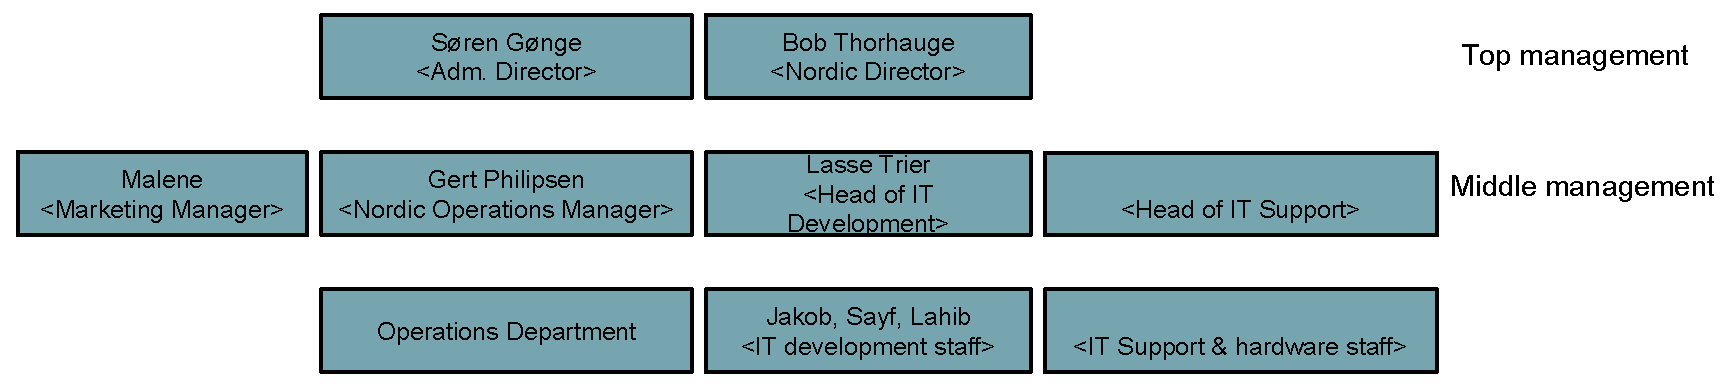
\includegraphics[scale=0.55]{img/Organizational_Chart}

\section{Key players}
This section describes the persons that have the most significant impact on the project.

\subsection{Lasse Trier}
Lasse Trier is the head of IT development. His main responsibility is to integrate customer’s IT systems and provide customer support when complications occur.\cite{lahib003}\cite{lahib004}\\
Additionally he prioritizes and delegates the tasks of three other employees of the development department.\cite{lasse009} He has an important role in providing competitive advantages to DANX as described in the Strategic Alignment Report in Work Domains. His impact on the project is significant, because he provides solutions to customer problems.

\subsection{Gert Philipsen}
Gert Philipsen is the head of the operational department. His responsibility is ensuring that DANX delivers on-time by coordinating and leading the operational department. He is concerned, among other things, with optimization of the operational department\cite{gert015}, which makes his opinion on the project important.

\section{Current work practices}
\label{sec:workpractices}
This section describes the work practices of the operational, IT development and IT support department that are relevant to the problem. The control tower is part of the operational department.\\
When customers of DANX wants to report a problem to DANX, they contact the control tower in the majority of cases.\cite{gert004} Customers can contact employees on other levels than the employees of the control tower.\cite{gert007} Customers can contact danx through phone or email, but mostly uses email.\cite{gert020} Each employee providing customer support has his own computer.\cite{gert024} The employee that receives the request might be able to solve the problem, if not, it is propagated.\\
The problems that the operational department can solve highly depend on the employee that takes care of the case.\cite{lasse002} Certain employees have knowledge of the problems related to EDI-connection and partially understand the format of the file that is transferred, and are able to solve some of them or identify the root cause. This is because Lasse has shared some of his IT knowledge with some of the employees of the operational department.\cite{lasse006} If the employee is not able to solve problem, it is propagated to the IT development department. Because some knowledge is acquired when trying to solve or identify the problem, it is in some cases propagated with a description, helping the IT development department solve it.\cite{gert006}\cite{lasse005}\\
The problems that are propagated to the IT departments are through the phone, email or delivered in-person.\cite{gert019} At least nine out of ten support requests are from the operational department.\cite{lasse001} If the responsible employee of the operational department is in doubt of which department is capable of solving the problem or do not know other means of contact, the email address it@danx.dk is used\cite{lasse003}. Both IT development and IT support have access to and check the email address, which makes coordination between the departments necessary.\cite{lasse004} This coordination is avoided if the employee of the operational department has sufficient knowledge of the responsibilities of the IT departments and the problem. In such a case, the private emails(e.g. ltr@danx.dk) or phones are used.\\
The IT development department usually solves problems related to customer integrations, because they make the integrations internally in the IT development department. Lasse Trier is the primary provider of support.\cite{lahib004} Other employees of the IT department helps integrating to some extent.\cite{lahib002}\cite{lahib003}\\
The IT support department solves problems related to hardware, for example dysfunctional PDA’s.\cite{lasse003}\\
Some problems from the same customer are recurring, because the problem was not solved in the first place.\cite{gert009}

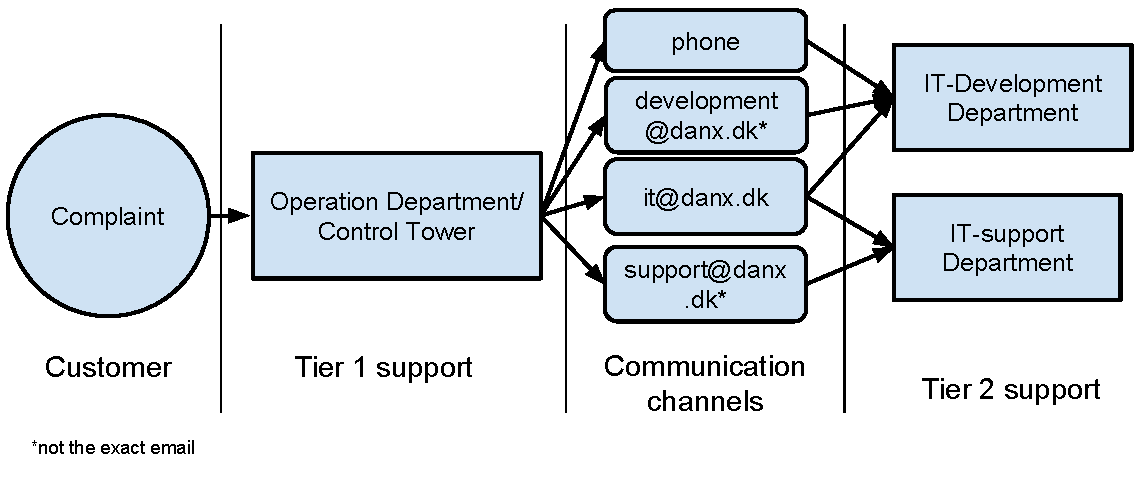
\includegraphics[scale=0.8]{img/Work_Practice_Flow}

\subsection{Stakeholder Analysis}
The purpose of the stakeholder analysis is to map the general interests of the key players with their role in the project.

\vspace{3mm}
\begin{tabular}{ | p{\dimexpr.18\textwidth-2\tabcolsep} || p{\dimexpr.41\textwidth-2\tabcolsep} | p{\dimexpr.41\textwidth-2\tabcolsep} | }
\hline
\rowcolor{GR}
\textbf{Stakeholder} & \textbf{General interests} & \textbf{Key interests and role in relation to the project}\\ \hline \hline
Operations department & Ensure that the delivery of spare parts is unhindered, by coordinating and integrating. & Providing effective customer support.\cite{gert016} Possibly part of the solution, because employees have knowledge of customer support. \\ \hline
Gert Philipsen & Ensuring that the operational department is functional and optimizing it. & Optimizing the operational department.\cite{gert015} As he leads the operational department his opinion on the project is important \\ \hline
Lasse Trier & On-time delivery of customer integrations and customer support & Lasse would like to document what customer support he has provided.\cite{lasse007}\\\hline
\end{tabular}

\section{Goals, Problems and Needs}
\label{sec:goalsproblemsandneeds}
This section describes the most significant goals and the problems that can hinder reaching the goals of the selected departments, or the goals described in chapter~\ref{chap:strategicalignmentreport}.
\subsection{Goals}
The IT department and the operational department has to integrate customers before their old contract expires. This can be everything between 1 day and to the 1st of next month.\cite{gert013}\cite{lasse008} It is important that the IT solution is ready on time, as DANX will not wait for the IT solution before they start working with the client\cite{lasse008}, this is to uphold the high service level. This means that if a system is not ready on time, DANX will start working with the customer without the IT system.\\
Not having an IT system results in additional workload because the data that the system creates and maintains automatically needs to be done manually. Fast integration is an important goal for the company because it makes the company fast in comparison to the competitors, some of which uses approximately 14 days for the integration. For reference see section~\ref{sub:competitor_analysis}\\
An important factor that makes DANX competitive, and therefore can be perceived as a goal, is that the customer can contact the IT department directly by email or phone avoiding the communication chain starting from the control tower. The problems that some customers of DANX experience can have serious consequences for their production or other practices that are hindered by the lack of a spare part.\cite{gert018} Having a shorter chain of communication and therefore a shorter response time can be a valuable service.\cite{lasse012}\\
These goals puts variable work pressure on the employees of the development department, because integration is a task that has to be done one time per customer, but takes at least an entire day. Customer problems are also varying.

\subsection{Problems}
There are several problems that can hinder the work practices that allows these goals to be reached. If the customer’s IT department is not ready on time, the integration can not be completed and DANX is forced to work without an IT system.\cite{lasse008}\\
In some cases the submitter of a customer problem is not clearly visible from the email containing the problem description. In this case the IT department spends from 10 to 15 minutes\cite{lasse013} on clarifying who the submitter of the problem is.\\
The IT support and IT development department spent time on reading mails that should be mailed to the other department because they share it@danx.dk.\cite{lasse010}\\
Internal support requests takes longer time to solve because of lacking information. The lacking information is retrieved by additional emails or phone contact.\\
The operational manager, can not supervise which customer support requests that are done and how long time it is pending. With this lack of knowledge it is complicated to optimize customer support. In the current situation, the knowledge of a specific problem can only be obtained by examining emails or talking to the employees that are responsible for solving the problem. The responsibility assignments are not documented, which complicates this further.\cite{gert012} The operational manager can not guarantee that a problem is solved within a given time period with no knowledge of the responsibility assignments.\\
With no documentation of customer support, KPIs of customer response time can not be established.\cite{gert011} The bigger DANX grow, the harder it is for a single manager to maintain an overview of how well the customer support is doing. As one of the goals of DANX is to grow, this issue becomes increasingly relevant.

\subsection{Needs}
The needs of the department is based on their current work practice, problems and the strategies identified in the Strategic Alignment Report.\\
The most important requirement for a solution to a problem within DANX is that it supports their rapid growth, because it is a business goal.\\
The SWOT analysis revealed that DANX has an advantages in direct customer support and fast integration, which the solution must keep or strengthen.\\
To keep the direct customer support, the solution can not change the way that customers contacts and communicate with DANX.\\
The IT development department has potential for optimization of work practices. A lot of the work that is done is information gathering that is necessary because the submitter of a problem has not included enough information, both for internal and external problems.\cite{lasse010}\\
As this increases the workload for the problem solver, providing this missing information can save time.\\
The solver of external problems is primary Lasse, and as he is responsible for much of the integration, support and prioritization of work, reducing his workload is a need. As DANX grows his workload will grow, because it is assumed that increasing the number of customers increases the number of support requests.\\
Both the IT development department and the operational department needs documentation of customer support in order to have data to base evaluation on. With no evaluation the operational manager can not know how well customer support is doing, and has no way to know where to optimize the department.\\
It is assumed that growth introduces additional employees and it is harder to asses an increasing number of employees’ performance without documentation. To guarantee that customer support requests are answered on-time, documentation that keep track of the request and the responsible employee is needed. It is assumed that an increasing amount of employees makes the need for employee evaluation increasingly important.

\subsection{Parallel projects}
The operation of DANX is educating their staff to understand the responsibilities of the different IT departments, such that they can submit the problem to the correct department, avoiding the responsibility overlap of it@danx.dk. In the future, the employees will preferable use the department-specific email, possibly decreasing the time that both departments uses on considering the problem.\cite{gert017}

\section{Ideas for solutions and suggested priorities}
\label{sec:ideas}
When trying to specify a solution it is important to be aware of what aspect of the problem that specific solution benefits, as a problem might require several solutions in order to be fixed.\\
Our focus is to provide DANX with means to generate documentation in a fast, efficient and uniform way, ultimately strengthening DANXs position in regards to keeping a high degree of service towards customers.\\

\subsubsection{First proposal}
Our first proposal is a simple software system with three main functions.\\
First it enables end-users(DANX employees) to keep track of support requests.\\
A request should contain information about the customer, description of the problem, the DANX employee handling the requests, the timestamps for when it was received, and when it was resolved.\\
Second it provides end-users with a filtering option to make sure that the data can be reviewed in an understandable fashion.\\
Third, since some support requests feature emails, it features a way to attach these to the requests.\\
This will give DANX documentation of how much support the IT-development department provides and how much the operations department provides, as well as the time spent providing it.\\
The time factor is a great addition, as this can be used to determine response times, and management is able to create KPIs eg. response time should be no greater than certain amount of days.\\
Furthermore the function of following up on unresolved tickets is a great tool for improving customer satisfaction.\\

\subsubsection{Second proposal}
The second proposal is in continuation of the first proposal.\\
It is similar to the first proposed system but it should additionally contain some extended information on the requests, particularly solutions to the problems and labels.\\
The labels should provide a means to group solutions into which types of problems they are.\\
An example of this could be the labels ‘EDI integration’ or ‘TrackIT integration’, providing end-users with a way to group possible solutions when providing support in certain fields.\\
When applying the second solution multiple benefits are achieved.\\
First and foremost, a well documented issue, which frequently occurs, might have a general solution for multiple customers, ultimately saving time spent on contacting experts within that particular field. \\
Secondly it might illustrate a flaw in the current practices, and the documented pattern can then be used to pinpoint the exact reason for the occurrence, which would make it easy for the experts to correct the issue or proactively attempt to avoid it.\\
In the second solution a crucial factor to success would be the fact that end-users of the system are provided with training in using the system and identifying problem types.\\
This is to ensure that they have the qualifications to tag the requests with their respective labelling.\\
This is important since the system would not function efficiently in regards to filtering if everything is mislabeled.\\
A downside to the second solution is that it will affect the time spent on initially handling the requests, seeing the employee has to manually write it into the system.\\
If an email has been sent it is possible to associate it with the request and save some time, but nevertheless one has to create the request.\\
When working with both solutions the parties affected directly would be the operations department and the IT development department.\\
This is due to the fact that these departments have first-hand contact with customers and are solving the customers problems.\\

\subsubsection{Customer impact}
Another important thing is that the systems are not to be forced upon the customers of DANX, as this might seem as a reduction in quality for them.\\
The system is intended to alter the workflow for the people answering the calls and the people handling the requests, and provide a structured way to review the work of the affected departments.\\
As Gert Phillipsen has expressed its important that solutions to problems are a part of the new system and hence we would recommend the second solution to have a higher priority.\cite{gert003}



\chapter{Solutions}
\label{chap:solutions}
\section{Requirements}
\textbf{R1} \\
The system must allow its users to create a ticket that includes information about:
\begin{itemize}
\item The person responsible for solving the problem or initially responsible for propagating the problem.
\item The customer and contact information, including preferable contact method.
\item Description of the problem and attached emails and/or files that relates to the problem.
\item Time and date of creation.
\end{itemize}

\textbf{R2} \\
The system must allow its users to edit the following information about a ticket:
\begin{itemize}
\item The description of a problem and attached files and/or email.
\item The customer, contact information and preferable contact method.
\item The person or department responsible for solving or propagating the problem.
\item Whether it is solved or not.
\end{itemize}

\textbf{R3} \\
When a problem has been propagated to a department or a person, the related person or department must be notified. \\

\textbf{R4} \\
The system must allow its users to browse tickets based on search parameters that are relevant to the evaluation of the customer support. \\

\textbf{R5} \\
The system must allow its users to create customer and supporter entities, such that when a ticket is created, an entity can be selected to avoid the need to write all of the information about a supporter or a customer. \\

\textbf{R6} \\
The system must have a login or another way of having a permanent identifier for whom the user of the running process is. This is to make responsibility assignment faster, as each employee providing customer support has his own computer.~\ref{sec:workpractices}

\subsection{Additional requirements}
\textbf{R6} \\
The system must allow its users to attach a solution to the ticket, and a label that identifies the problem. The solution must be able to include both text, files and emails. \\

\textbf{R7} \\
The system must allow its users to browse solutions based on search parameters, that includes the label that identifies the problem.

\section{Finances}
\subsubsection{Benefits}
\textbf{Customer loss avoidance}
Customer loss avoidance is calculated the same way in each of the 3 analysis. Based on the information\cite{bob004} we received from Bob the cost of implementing a new customer is 15,000 DKK for IT, 30,000 DKK for marketing and 40,000 DKK for operation. This is a total of DKK 85,000. Based on the assumptions in the assumption section~\ref{subsub:assumptions} we have included a profit of 85,000 each year. \\

\textbf{Faster solution to problems}
Faster solutions to problems is calculated the following way:
\[ 50 \frac{\mathrm{request}}{\mathrm{week}} \times 52 \frac{\mathrm{week}}{\mathrm{year}} \times 0.5 \frac{\mathrm{hour}}{\mathrm{request}} \times 200 \frac{\mathrm{kroner}}{\mathrm{hour}} \times 0.02 = 5200 \frac{\mathrm{kroner}}{\mathrm{year}} \]
50 requests/week * 52 weeks/year * half an hour (0.5) / request * 0.02 (2\% of the requests can be solved due to the already existing solutions) * 200 DKK/hour. See the assumptions in section~\ref{subsub:assumptions}.
This is however not included in the basic tailored solution since the solution to a problem is not documented.
This ends up as 5200 DKK which is another positive number for the first year. As seen in the assumptions section~\ref{subsub:assumptions} the number grows with 2\% each year. This is due to the number of solutions to problems becoming larger each year.\\

\textbf{More sale}
As seen in section~\ref{subsub:assumptions} DANX is able to gain an additional customer each year, resulting in DANX receiving an additional 2.65 millions each year. This is not included in the initial/investment year since there will be no documentation for the KPIs that year. \\

\textbf{Less time writing emails}
Currently the operation spends time writing emails and/or rephrase emails before it is sent to the IT development department \cite{gert006} \cite{lasse003}. With the new system there is no longer a need to do this, as the request will already be written in a ticket. This is calculated as 50 requests/week * 52 weeks/year * 5 min/request * 1/60 (to convert it to hours) * 200 hourly rate.
\[ 50 \frac{\mathrm{requests}}{\mathrm{week}} \times 52 \frac{\mathrm{week}}{\mathrm{year}} \times 5\frac{\mathrm{minute}}{\mathrm{request}} \times \frac{1}{60} \frac{\mathrm{hour}}{\mathrm{minute}} \times 200\frac{\mathrm{kroner}}{\mathrm{hour}} \approx 43,333 \frac{\mathrm{kroner}}{\mathrm{year}} \]
This comes out as 43.333, which is the same every year.

\subsubsection{Cost}
\textbf{Initial investment}
The initial investment differs from solution to solution. They are based on the price of Kayako\cite{webpage008} Since 6 users from the operation\cite{gert014} department and 2 users from the IT department\cite{lahib003} will be using the system the price is DKK 16.242 for the off-the-shelf solution at the time of writing. The tailored extended system will thus be 16.242 * 3 as described in the assumption section~\ref{subsub:assumptions} which is DKK 48.726 and the basic is 16.242 * 2,5 which is 40.605.\\

\textbf{Staff training}
It is assumed~\ref{subsub:assumptions} that it takes 5 hours per employee for the basic system, 6 hours for the extended system, and an additional 20 hours for the kayako system. The total cost is calculated the following way:
\[ 5 \frac{\mathrm{hour}}{\mathrm{employee}} \times 8 \hspace{1mm} \mathrm{employee} \times 200 \frac{\mathrm{kroner}}{\mathrm{hour}} = 8,000 \hspace{1mm} \mathrm{kroner} \]

\[ 6 \frac{\mathrm{hour}}{\mathrm{employee}} \times 8 \hspace{1mm} \mathrm{employee} \times 200 \frac{\mathrm{kroner}}{\mathrm{hour}} = 9,600 \hspace{1mm} \mathrm{kroner} \]

\[ \left( 6 \frac{\mathrm{hour}}{\mathrm{employee}} \times 8 \hspace{1mm} \mathrm{employee} + 20 \hspace{1mm} \mathrm{hour} \right) \times 200 \frac{\mathrm{kroner}}{\mathrm{hour}} = 13,600 \hspace{1mm} \mathrm{kroner} \]
5 hours * 8 employees * an hourly rate of 200 which is 8.000 for the basic system, 9.600 for the extended system and 13.600 for the off-the-shelf solution. \\

\textbf{Support/Updates}
Support and updates for kayako is 40\% off the initial price. For the Tailored systems it is 25\% as seen in section~\ref{subsub:assumptions}. For kayako this is 6.497. The tailored extended system is 12.182 and the basic tailored system is 10.151.\\

\textbf{Additional time spent on documentation}
It is assumed~\ref{subsub:assumptions} that for the extended system and kayako it takes 14 minutes to document a request, and 7 minutes for the basic system.
So to calculate the extended version we use:
\[ 50 \frac{\mathrm{request}}{\mathrm{week}} \times 52 \frac{\mathrm{week}}{\mathrm{year}} \times 14\frac{\mathrm{minute}}{\mathrm{request}} \times \frac{1}{60} \frac{\mathrm{hour}}{\mathrm{minute}} \times 200\frac{\mathrm{kroner}}{\mathrm{hour}} \approx 121,333 \frac{\mathrm{kroner}}{\mathrm{year}} \]

\[ 50 \frac{\mathrm{request}}{\mathrm{week}} \times 52 \frac{\mathrm{week}}{\mathrm{year}} \times 7\frac{\mathrm{minute}}{\mathrm{request}} \times \frac{1}{60} \frac{\mathrm{hour}}{\mathrm{minute}} \times 200\frac{\mathrm{kroner}}{\mathrm{hour}} \approx 60,666 \frac{\mathrm{kroner}}{\mathrm{year}} \]

50 requests/week * 52 weeks/year * 14 min/request * 1/60 to convert minutes to hours * an hourly rate of 200 which is 410.982 in total. For the basic  system 14 is replaced by 7, and the new total is 266.157
The documentation is required all years including the initial (investment) year and remains consistent. \\

\textbf{Additional time spent on analysing}
As seen in the assumptions section~\ref{subsub:assumptions} Gert is responsible for conducting the analysis. To calculate the yearly cost the following formula is used:
\[ 1 \frac{\mathrm{analysis}}{\mathrm{week}} \times 52 \frac{\mathrm{week}}{\mathrm{year}} \times 1 \frac{\mathrm{hour}}{\mathrm{analysis}} \times 300 \frac{\mathrm{kroner}}{\mathrm{hour}} = 52,840 \frac{\mathrm{kroner}}{\mathrm{year}}\]
1 analysis/week * 52 weeks/year * 1 hour analysis * an hourly rate of 300. This equals 52.840 and is the same for all systems and every year, except the initial/investment year, which is 0 as not enough data has been recorded.

\subsection{Assumptions}
\label{subsub:assumptions}
It is assumed that DANX can save one customer each year by using the new system. This is due to DANX is able to analyse their customer support service, and thus provide better quality and service, which helps keeping the customers. This does not include the initial investment year, as it is not expected that DANX has built a large enough knowledge base based on answers to previous requests, thus not able to provide a better service yet.\\
DANX expect to grow with 25-30 customers a year.\cite{bob003} Some of potential customers requests the customer support KPIs and if DANX is unable to show these, they may lose that customer. Our system enables DANX to show the support KPIs thus getting 1 customer each year. The income of a customer is based on DANX expects to grow with additional 250 million in 3-4 years, they get 25-30 (27) customers each year, and to see what this brings us in one year we divide with 3,5 years, which results in 2.65 millions\\
It is expected that the number of solutions to problems grow each year. Therefor the number of requests that can be solved by a quick search in the solution is expected to climb with 2 percent point each year (for the first 4 years). \\
The initial investment for the tailored extended system is expected to be 3 * the price of kayako since it is a new system that needs to be written from scratch. The basic version is only expected to be 2,5 * the price of kayako as it is more simple and has less functionality. \\
Staff training is expected to be 5 hours per employee on the basic solution and 6 hours on the extended solution. On kayako there is a kayako query\cite{webpage009} language (programming language) that needs to be learned from the IT development department in order to generate the reports used when analysing data. This is expected to be an additional 20 man hour.
It is also expected that the employees trained in the system have an hourly rate of 200 DKK.\\
Support/Updates are only expected to be 25\% of the initial investment for the tailored systems. This is due to the system is tailored and that you already paid a larger sum for the initial investment than with the off-the-shelf solution. It is assumed that the first year of support and updates for the tailored systems is free. \\
Additional time spent on documentation varies from the basic to the extended solution. This is because you have to document the solution in the extended version and this means that the employees have to spend more time on each request.
Therefore it is assumed that if one is using the basic system the time required will be 7 minutes, and 14 minutes if using the extended solution. 
It is expected that Gert carries out the analysis, and analyse one report each week, spending 1 hour at it, and has an hourly rate of 300. \\

\section{Implementation strategy}
\label{sec:implementation_strategy}
This section describes the recommended implementation strategy. The purpose of this is to have a structured approach for integrating the proposed system.\\
In regards to the tailored systems an additional factor is taken into account, the system development.\\
If the development phase is not properly controlled its a high risk factor, this is due to the different aspects that can go wrong during the development, this includes but is not limited to misinterpretation of software specifications and miscommunication between suppliers and customers.\\
During the development of the new system, it is important to continuously ensure the quality of the system. This means that some DANX employees are going to spend time evaluating the new system, via mockups and/or prototypes and confirm that it is heading in the right direction. \\
It is important to do the evaluations, in order to make sure that the system meets the requirements and is understandable to the employees of DANX.\\
It is important to note that the requirements we have provided earlier are not complete, they are on an abstract level, which means that some additional specification is required when actually developing.\\
If the development is done inhouse at DANX it is important to keep in mind the added strain on the IT development department. If DANX is not aware of this, the risk of the development falling behind, either in time or quality, is significant. \\
Another important aspect to consider when choosing tailored systems developed out of the house, is whether to request the supplier to hand over all source code of the system to the IT department of DANX.\\
If the source code is supplied, it ensures that DANX will be able to maintain and develop the system, this obviously puts additional strain on the IT development department.\\

\textit{The above only applies to the tailored systems, the following is general for all three systems.}

When DANX is about to roll out a system, there are several approaches to be considered.\\
Firstly it is possible to make an all out installment of the system. This means that over a short time gap, all employees who are supposed to use the system, should have it available at their workstation and be able to use it from that moment.
This has the advantage of being incredibly fast and easy - fast in the sense that it will be a simultaneous rollout to all workstations, easy in the sense that when rolling out to all users at once implications where some of the affected staff is not able to access ‘new’ data is avoided.\\
On the other hand it contains a higher risk, because if some aspect of the integration goes wrong, all included departments will most likely experience the errors.\\
Secondly it is possible to roll out the system incrementally. This is done by choosing a group of employees who are going to use the system and gradually increase the amount of employees using the system.
The advantage gained is that only some employees will need support initially and gradually as more employees start to use the system, the requested IT support can be  provided by  colleagues who have already used the system for some time.
On the other hand this process is slow and results in creating several workflows.\\
During the time where only some employees use the system, employees with and without the system will have to do something different in their work practices, this will trouble communication in and between departments.\\
Before the deployment of the system, all employees will have to receive training in how to use the system, as described in\ref{subsec:qualification}. These training sessions should be planned as close to the deployment of the system, in order to prevent employees from forgetting too much before they start using the system and to minimize the scenario of radical changes being implemented in the system.\\
There are two ways to conduct the training. Either a full seminar where all the staff of the affected departments is attending or train a few employees in every department and have them train the others.
Since DANX has a 24/7 hotline(operations department), its not sustainable to pull this department out for training. Neither is it possible to pull out all IT staff at once either, since this cripples the support.
Therefore in regards to our two proposed ways of conducting training, taking out a few employees for training, and have them train others seems as the best solution.

\chapter{Figures}

\section{Slide from a DANX presentation}
\label{sec:slide_from_DANX}
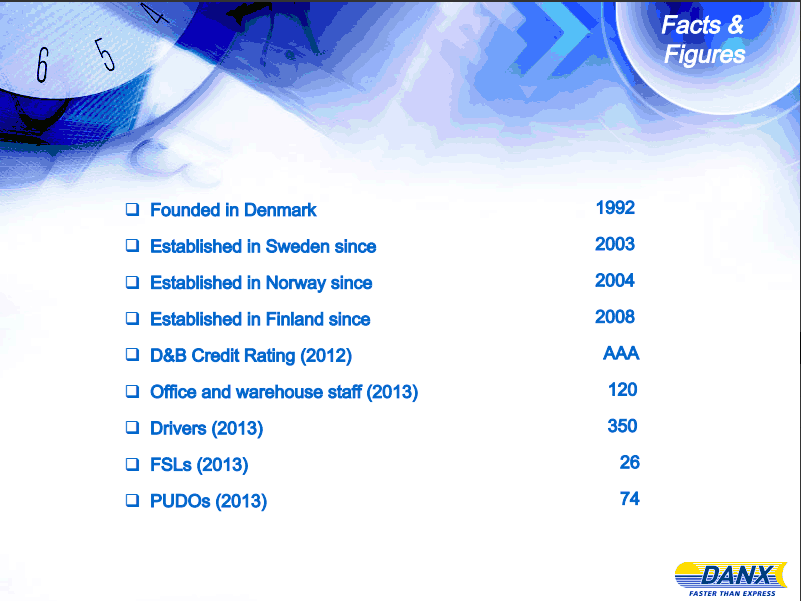
\includegraphics[width=\textwidth]{img/DANX_FSL_PUDO}
%http://i.imgur.com/VcV07XS.png


\section{Cost benefit for tailored basic solution}
\label{sec:cost_tailored_basic}
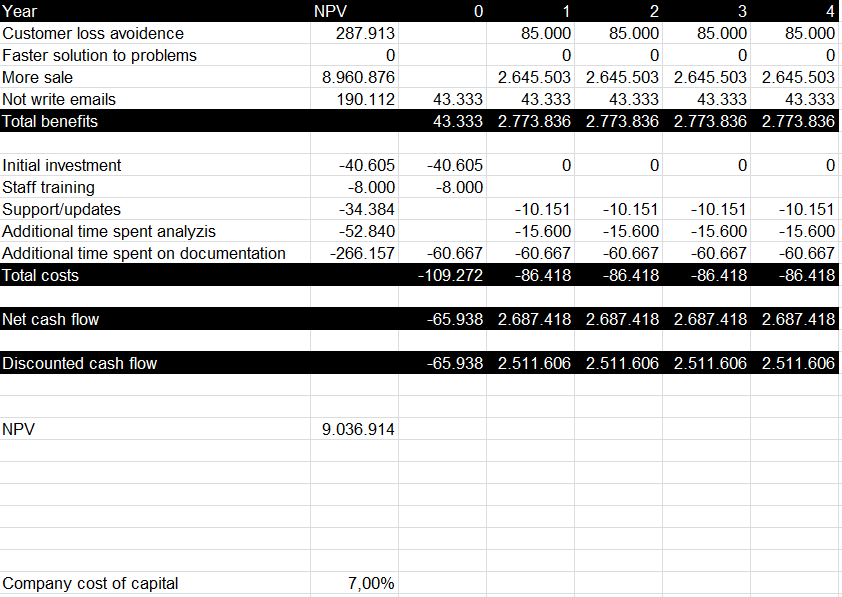
\includegraphics[width=\textwidth]{img/CostBenefit_TailoredBasic}
%http://i.imgur.com/rJZnQZi.png


\section{Cost benefit for tailored extended system}
\label{sec:cost_tailored_extended}
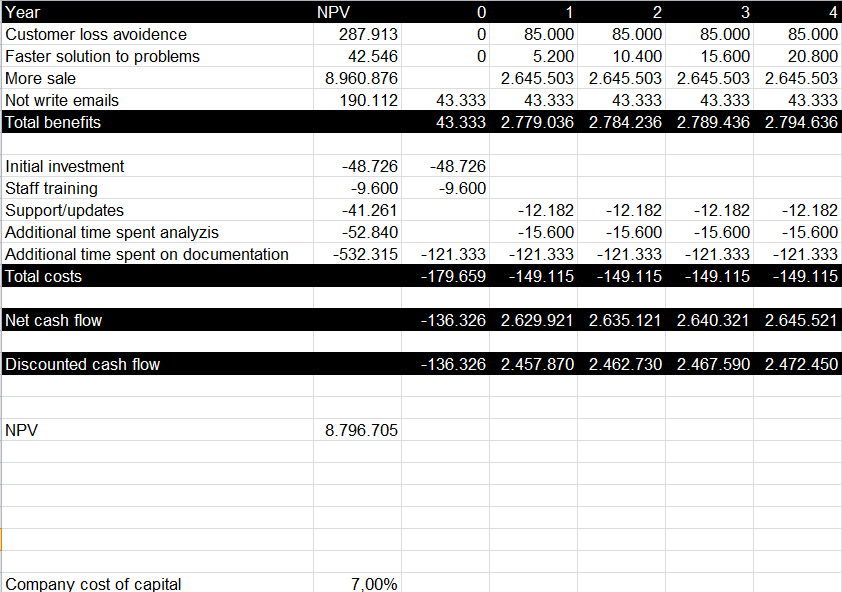
\includegraphics[width=\textwidth]{img/CostBenefit_TailoredExtended}
%http://i.imgur.com/iNIannt.png


\section{Cost benefit for off-the-shelf solution kayako}
\label{sec:cost_off-the-shelf}
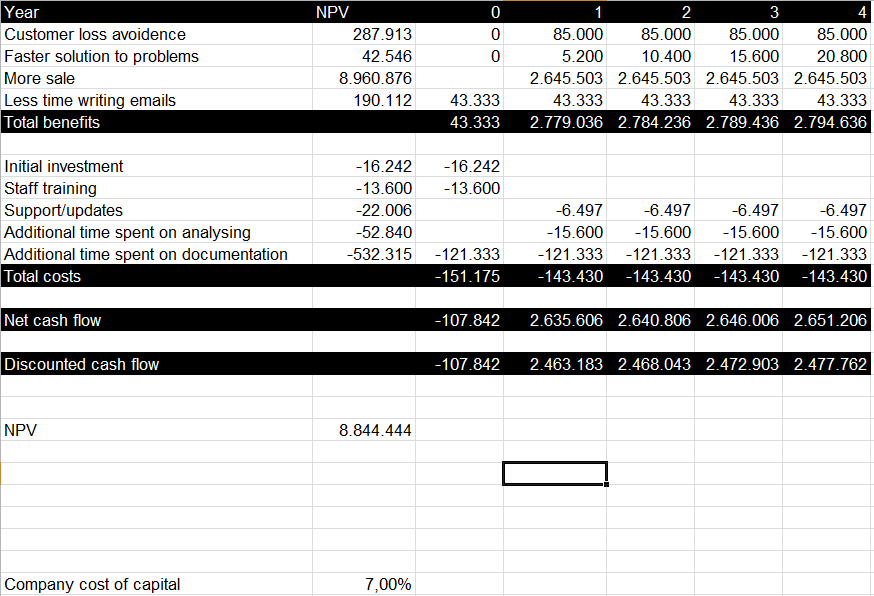
\includegraphics[width=\textwidth]{img/CostBenefit_Off-the-shelf}
%http://i.imgur.com/bUaRjPM.png

\section{Business Canvas}
\label{sec:business_canvas}
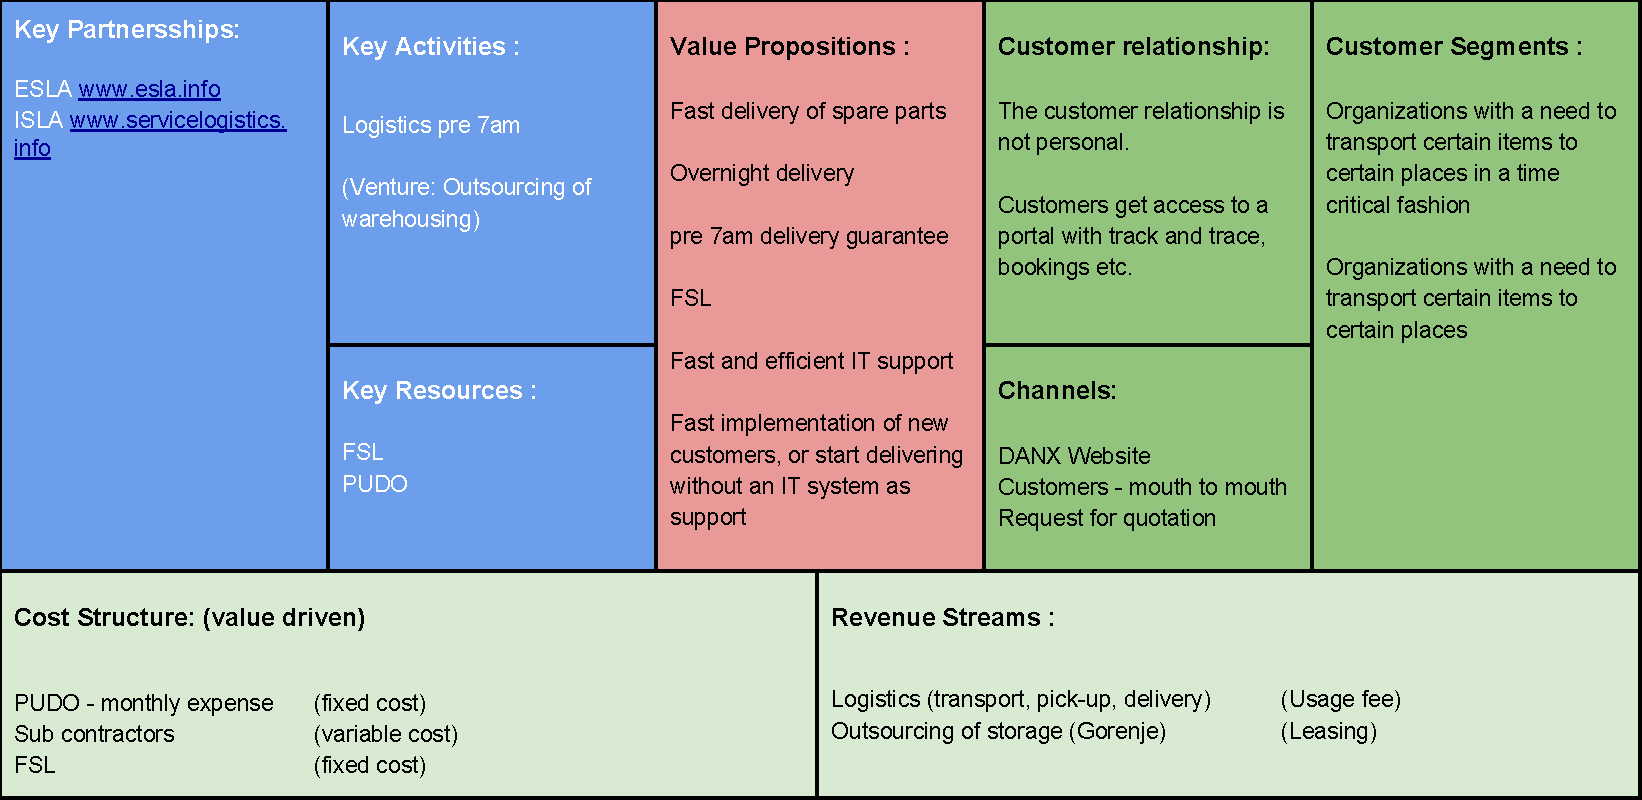
\includegraphics[angle=270, scale=0.85]{img/Business_Canvas.pdf}

\end{appendices}

\begin{thebibliography}{9}

\bibitem{gert001}
	Malene(0 - 21:03), Gert(21:03 - 1:13:20) \& Lasse(1:13:20 - slut).3ga - Time 24:47\\
	\textit{[...] vi henter jo hver dag nede i Holland og leverer i hele Danmark inden 7.}

\bibitem{gert002}
	Malene(0 - 21:03), Gert(21:03 - 1:13:20) \& Lasse(1:13:20 - slut).3ga - Time 43:00\\
	\textit{[...] hente nede i Salzgitter som ligger nede syd for Hannover klokken 15:30 og så samtidig levere oppe nord for Stockholm inden 7 næste morgen.}

\bibitem{gert003}
	Gert \#2 2/2.3ga - Time 02:17\\
	\textit{[...], så skal man altså også have løsningsdelen med, hvornår det er løst og sådan, før det har en værdi der. Og hvis man ikke gør det, så føler jeg at det mister meget af sin værdi.}

\bibitem{gert004}
	Gert \#2 1/2.3ga - Time 03:10\\
	\textit{[...] og hvis de ringer til vores hovednummer er det control tower de får, så det er jo egentlig der den meste kontakt foregår}

\bibitem{gert005}
	Gert \#2 1/2.3ga - Time 04:15\\
	Om kontroltårnet selv løser problemer for kunder: \textit{Det kunne sagtens være, der hvor kunden siger noget, kan vi godt sige til dem, jamen prøv at hør, hvis du nu går ind på vores hjemmeside, så kan du gøre sådan og sådan}

\bibitem{gert006}
	Gert \#2 1/2.3ga - Time 06:21\\
	\textit{Hvis jeg får noget fra en intern eller en kunde prøver jeg på en eller anden måde at oversætte det sådan at det er mere klart defineret når det kommer til IT}

\bibitem{gert007}
	Gert \#2 1/2.3ga - Time 03:30\\
	\textit{\emph{(rd: om kunden)} som så skyder det ind på et andet niveau her, for eksempel ved at kontakte mig eller Bob, eller et andet niveau altså}

\bibitem{gert009}
	Gert \#2 1/2.3ga - Time 14:45\\
	Om de får den samme support request flere gange: \textit{Hvis du får den samme forespørgsel flere gange så er det jo en rykker, enten fordi vi snakkede om det dengang eller fordi vi ikke lige har fået set på det, og det så bliver nævnt igen. Også siger vi jo det skal vi nok prøve at se på eller komme tilbage til også er vi ikke lige kommet tilbage.} Interviewer: \textit{Hvad er årsagen til det?} \textit{Det er fordi hvis jeg sender en mail til Lasse så er det ikke sikkert jeg husker at følge op på det, og hvis han ikke svarer, så husker jeg det først når kunden rykker på mig, så vi mangler et struktureringsværktøj. }

\bibitem{gert010}
	Malene(0 - 21:03), Gert(21:03 - 1:13:20) \& Lasse(1:13:20 - slut).3ga - Time 1:08:10\\
	Interviewer: \textit{Kan du fortælle lidt om ESLA?}\\
	Gert: \textit{Ja og det er også det partnerskab vi har, det er ESLA.}\\
	\textit{[...] Vi går ud og markedsfører og sammen og hvis vi får en kunde der vil bruge den samme, jamen så kan vi snart gå ud og dække en stor del af Europa med det samme tilbud.}\\
	\textit{[...] og bruge hinanden også har meget, vi vil være gode venner og vi supporter hinanden hvis der er et eller andet vi kan hjælpe hinanden med det gør vi meget for at gøre. Har meget open books, de må gerne komme op og se alt hvordan vi producerer, jeg må gerne komme ned og se hvordan de producerer, jeg har så ikke fået gjort det endnu.}

\bibitem{gert011}
	Gert \#2 1/2.3ga - Time 18:05\\
	Interviewer: \textit{Har i egentlig nogen KPIer i forhold til svartider?}\\
	Gert: \textit{Nej, slet ikke, overhovedet ikke. Det har vi ikke.}

\bibitem{gert012}
	Gert \#2 1/2.3ga - Time 18:20
	Om customer support:
	\textit{Vi har ingen form for dokumentation på det.}

\bibitem{gert013}
	Gert \#2 1/2 - Time 21:11
	\textit{Nu her er vi blevet bekræftiget i at vi skal starte en stor kunde op i danmark og sverige og de skal starte her den første januar, jamen så integrerer vi til den første januar.}

\bibitem{gert014}
	Telefonopkald med Gert\\
	Interviewer: \textit{Ved du ca. hvor mange der arbejder i operationen?}
	 Gert: \textit{I operationen og i control tower er der seks mennesker.}

\bibitem{gert015}
	Telefonopkald med Gert\\
	Interviewer: \textit{Ser du en af dine primære interesser, som at være optimering af operationen?} Gert: \textit{Ja, helt klart.}

\bibitem{gert016}
	Telefonopkald med Gert\\
	Interviewer: \textit{Ser du en af operationens interesser som at være at give effektiv customer support?} Gert: \textit{Ja, det tror jeg også at jeg vil sige ja til.}

\bibitem{gert017}
	Gert \#2 1/2.3ga - Time 10:06\\
	\textit{Jamen, egentlig har det været it@, men nu har de delt dem op og de har også lavet en der hedder support@danx.dk og development, vi har bare ikke spredt rygtet om det endnu, og vi har faktisk haft et møde i dag om med de forskellige operationschefer i de forskellige lande, hvor vi havde lasse med inde for at få noget struktur over det. [...] Så det er klart at der skal være en mail kun til dem og den er vist også ved at blive fabrikeret og publiceret. }

\bibitem{gert018}
	Malene(0 - 21:03), Gert(21:03 - 1:13:20) \& Lasse(1:13:20 - slut).3ga - Time 25:50\\
	\textit{Under høsten der er det jo sådan at en landmand, der ser vejrudsigten, “nu er det altså i morgen jeg skal høste”, også ryger kniven på hans mejetærsker, så vil han altså have den ud og køre i morgen}

\bibitem{gert019}
	Gert \#2 1/2.3ga - Time 08:41\\
	\textit{Jeg sidder jo her hvor jeg sidder, så nogle gange går jeg ind til ham\emph{(rd: Lasse)}, nogle gange sender jeg en mail, og det er ret sjældent jeg ringer til ham.}

\bibitem{gert020}
	Gert \#2 1/2.3ga - Time 12:54\\
	Interviewer: \textit{Hvis du kunne lave et skøn, de henvendelser I får fra kunden som ikke er fra statusmøder, hvor mange af dem er skriftlige og hvor mange af dem er mundtlige?} Gert: \textit{Der vil jeg tro at langt de fleste er skriftlige.}

\bibitem{gert021}
	Malene(0 - 21:03), Gert(21:03 - 1:13:20) \& Lasse(1:13:20 - slut).3ga - Time 29:21\\
	Interviewer: \textit{Jeg kunne forstå i bruger fly udelukkende til blandt andet Helsinki, har i så samarbejde med flyselskaberne sådan at i sikrer at der er plads til jeres var der skal leveres}\\
	\textit{[..] Fly selskaber vil primært transportere passagere, så uanset hvad vil der indgå en situation hvor et fly er sent på den, og så siger kaptajnen, for han vil gerne flyve til tiden, så siger han, vi tager ikke noget fragt med i dag.}

\bibitem{gert022}
	Malene(0 - 21:03), Gert(21:03 - 1:13:20) \& Lasse(1:13:20 - slut).3ga - Time 50:47\\
	Interviewer: \textit{Vi er interesseret i at vide noget om jeres struktur, hvilke afdelinger i har og hvordan de snakker sammen.}\\
	Gert: \textit{Hvert land har en landechef, hvert land har også en ansvarlig for operationen, og hvert land har faktisk også, undtagen Norge, en sælger, altså en der er tilknyttet vores salgsafdeling. Og det er jo klart at det er landecheferne der er ansvarlige for at deres land fungere både operationelt og administrativt og med legale, personale og alt sådan noget der og salgsmæssigt. Og så har vi alligevel valgt at have en nordisk operationsafdeling som jeg så leder [..] Så har vi en nordisk salgsafdeling. [..] Vores IT er nordisk og ligger her i vallenspæk. }

\bibitem{gert023}
	Malene(0 - 21:03), Gert(21:03 - 1:13:20) \& Lasse(1:13:20 - slut).3ga - Time 41:59\\
	Gert: \textit{PUDO’er er sådan en ting, som er customer driven, altså kundernes behov, altså det der har fået os til at åbne måske 28 PUDO’er i sverige er fordi IBM vil have PUDO’er og HP vil have PUDO’er og [Bincoy Neksdov] vil have PUDO’er, så åbner vi alle de der PUDO’er i sverige. Så det er jo klar, det er også med til at styrke os. Og nu er det så vigtigt for os at få flere kunder ind på PUDO’erne, for sådan nogle PUDO’er har typisk en fast månedlig omkostning. Som helst skal være så lille så muligt, og alligevel skal vi have så meget så muligt gennem PUDO’erne.}

\bibitem{gert024}
	Telefonopkald med Gert\\
	Interviewer: \textit{Har alle der giver customer support deres egen computer?} Gert: \textit{Ja, det har de.}

\bibitem{gert025}
	Malene(0 - 21:03), Gert(21:03 - 1:13:20) \& Lasse(1:13:20 - slut).3ga - Time 39:12\\
	Interviewer: \textit{Hvordan prøver i at adskille jer fra jeres konkurrenter? Altså hvorfor vælger kunden jer frem for en anden?} Gert: 	\textit{Der hvor vi prøver og altid har prøvet at stå lidt for os selv, det er at vi har en høj kvalitet og vi gør meget for at have en høj kvalitet.}

\bibitem{gert026}
	Malene(0 - 21:03), Gert(21:03 - 1:13:20) \& Lasse(1:13:20 - slut).3ga - Time 39:12\\
	Interviewer: \textit{Hvordan måles denne her branche sig på kvalitet?} Gert: 	\textit{Det er levering til tiden, og ved forsinkelser, årsagen til den.}

\bibitem{gert027}
	Malene(0 - 21:03), Gert(21:03 - 1:13:20) \& Lasse(1:13:20 - slut).3ga - Time 40:10\\
	Gert: \textit{[...] der vil aldrig nogensinde stå i en oplysning fra os til kunden at vores bil er punkteret for eksempel. Det kan godt være vi har et technical breakdown, men det er sjældent. Hvis vi har et problem og vi kan nå, ved at bruge nogle penge, og så stadig levere til tiden, så gør vi det. Så vi investerer meget backup omkostninger i at holde vores høje kvalitet.}

\bibitem{gert028}
	Malene(0 - 21:03), Gert(21:03 - 1:13:20) \& Lasse(1:13:20 - slut).3ga - Time 51:07\\
	Gert: \textit{Jamen, du kan sige, vi er en ret flad organisation. Vi har afdelinger i alle landene.}

\bibitem{bob001}
	\textit{Nogle potentielle kunder vil gerne se support KPIer.}

\bibitem{bob002}
	\textit{Nogle kunder kræver referencer fra andre kunder.}

\bibitem{bob003}
	\textit{Dvs at vi fokusere på at vokse med ca. 25-30 om året i organisk vækst \emph{(rd: nye kunder)}}\\
\textit{Sidst eår tjene vi ca 10 mill indne skal, hvilket er for lidt ud af 250 mill i omsætning. I indeværende år (13/14) kommer vil til at omsætte plus 300 mill og et overskud på plus 20 mill før skat.}\\
\textit{Overordnede sigter jeg mod at DANX om 3-4 år har en omsætning på plus 500 mill med et overskud på ca 8-10 procent. Det vil give en potentiel salgsværdig på + 500 mill.}

\bibitem{bob004}
	Hvor meget koster det ca. at implementere en ny kunde?
	\textit{“Jeg vil skyde på at det koster 15000 it-mæssigt, 40000 operationelt og 30000 salgsmæssigt.”}

\bibitem{malene001}
	Malene(0 - 21:03), Gert(21:03 - 1:13:20) \& Lasse(1:13:20 - slut).3ga - Time 09:23\\
	\textit{[...] nogen af vores største konkurrenter er TNT og HIT}

\bibitem{malene002}
	Malene(0 - 21:03), Gert(21:03 - 1:13:20) \& Lasse(1:13:20 - slut).3ga - Time 04:30
	\textit{Søren gønge, som er ham der grundlagde firmaet, er ham der ejer mest også har Bob også en stor del af aktierne, også alle tre country managers der sidder i norge, sverige og finland ejer også en del af virksomheden.}

\bibitem{opemployee001}
	\textit{“Vi har på nuværende tidspunkt en hel reol stående med ringbind til de 19 systemer som vi benytter i forbindelse med vores kundesystemer”}

\bibitem{lahib001}
	Lahib.3ga - Time 13:00\\
	\textit{[...] så jeg programmerede noget 3 måneder siden og fuldstændig glemt hvordan fanden jeg havde lavet det. Så jeg skulle gå helt tilbage og justere det eller faktisk skrotte det fuldstændig og lave noget helt ny implementering.}

\bibitem{lahib002}
	Lahib.3ga - Time 00:51
	\textit{Min opgave har så været, for 3-5 kunder at få forbindelse til en ftp eller en sftp server hvor jeg kan hente filerne, arkivere dem også bagefter uploadede dem, så det er både upload og download og arkivering af filerne.}

\bibitem{lahib003}
	Lahib.3ga - Time 17:42
	\textit{Hvorimod Lasse han har direkte kontakt med kunden, hvor kunden siger “Det her, jeg har seks filer der ikke er kommet i dag, hvad er der sket, de her filer er ikke blevet importeret fra vores til jeres server.” Så jeg vil sige, Lasse ja, og Jakob lidt, men mig og Safe vi får ikke så mange \emph{(rd: customer support requests)}.}

\bibitem{lahib004}
	Lahib.3ga - Time 17:09
	\textit{Lasse får sindsygt meget(support requests) hver dag. Jeg gør ikke, Safe gør heller ikke, Jakob gør lidt, mere end mig.}

\bibitem{lasse001}
	Lasse \#5.3ga - Time 15:25 \\
	Interviewer: \textit{Hvor ofte er operationen mellemled for support henvendelser fra kunden?} Lasse: \textit{Stort set altid, vi snakker 90\% af gangene i hvert fald}

\bibitem{lasse002}
	Lasse \#5.3ga - Time 8:27 \\
	Til om nogen fra operationen kan løse it-problemer: \textit{Det er igen lidt et tilfælde hvem der kan det og ikke kan det.}

\bibitem{lasse003}
	Lasse \#5.3ga - Time 16:08 \\
	\textit{Jeg har jo lidt et problem eller en udfordring med ved at vi har to afdelinger både en IT support og en IT development, og de sender jo bare til @it som har begge afdelinger blandet sammen så vi for jo en masse mails hvis der er for eksempel problemer med PDA’erne eller et andet hvor det sådan set ikke er min afdeling, så vi får en masse clutter-mail på grund af det her.}

\bibitem{lasse004}
	Lasse \#5.3ga - Time 17:10 \\
	\textit{Hvis de andre har travlt så svarer vi jo også, vi hjælper jo hinanden \emph{(rd: IT afdelingerne)}}

\bibitem{lasse005}
	Lasse \#5.3ga - Time 18:30 \\
	Interviewer: \textit{Hvor de(operationen) har korrespenderet med en kunde?} Lasse: \textit{Ja, men hvor de så også skriver hvad det er der er problemet.}

\bibitem{lasse006}
	Lasse \#5.3ga - Time 21:35 \\
	\textit{Jeg har jo lært for eksempel haydar\emph{(rd: ansat i operationen)} at gå ind at kigge i EDI filen hvis der er fejl advisering eller et eller andet så han kan gå ind og se for vi gemmer dem et bestemt sted og han er begyndt at kunne gennemskue de fleste af dem, altså se hvordan ser denne her forsendelse egentlig ud, så han har taget meget af det jeg har siddet og gennemtrawlet og se om de har sendt den her forsendelse gennem de rigtige kanaler, er den i vores fil og i så fald hvad er der så gået galt.}

\bibitem{lasse007}
	Malene(0 - 21:03), Gert(21:03 - 1:13:20) \& Lasse(1:13:20 - slut).3ga - Time 01:50:38
	\textit{Nogle gange kunne det være meget rart for mig at sige, prøv at se her hvor meget vi egentlig har lavet, og her kunne et ticket system jo være meget relevant.}

\bibitem{lasse008}
	Lasse \#5.3ga - Time 03:13 \\
	\textit{Hvis ikke IT integrationen er færdig, jamen så kører vi ud med pakkerne alligevel, altså så gør vi det uden. Så vi kan som regel integrere en ny kunde, hvis de er klar, inden for en til to dage.}

\bibitem{lasse009}
	Malene(0 - 21:03), Gert(21:03 - 1:13:20) \& Lasse(1:13:20 - slut).3ga - Time 02:05:38
	Om hvordan arbejdet bliver struktureret \textit{Vi holder møder, jeg holder ugentlige møder, nogen gange er det hver 14 dag eller en gang om måneden, det kommer lidt an på hvor meget stress der er på, men hvor at, altså vi har ikke noget task system eller management system, så det bliver meget lister, hvor jeg siger “nu vil jeg gerne have en liste på alt det der mangler i det her system” også sidder jeg og prioriterer hvad der er vigtigt og hvad der er knap så vigtigt.}

\bibitem{lasse010}
	Lasse \#2.3ga - Time 08:30\\
	\textit{[...] ofte så bruger folk ikke de der 5 minutter på at skrive en mail og skrive præcis hvad problemet er, så det ender med en mailkorrespondance på 5 mails frem og tilbage, for at finde ud af hvad problemstillingen er.}

\bibitem{lasse011}
	Lasse \#2.3ga - Time 20:10\\
	\textit{Jeg har snakket med i hvert fald 10 og det var kun inden for IT området, altså der var også alt det praktiske. Der er det jo smart at der er 10 mennesker der kan snakke med mig, altså jeg ved alt det 10 mennesker ved på deres side.}

\bibitem{lasse012}
	Malene(0 - 21:03), Gert(21:03 - 1:13:20) \& Lasse(1:13:20 - slut).3ga - Time 01:18:32
	\textit{Jeg synes det fungerer rigtigt godt, jeg synes vi har en fordel i forhold til nogle af de andre firmaer, at de\emph{(rd: kunder)} kan komme i kontakt til os direkte, at vi ikke har et support system og et 4 tiers call desk hvor at man skal igennem de første tre der ikke ved noget som helst, som nogle af vores konkurrenter har, og det er en fordel, og det ser vores kunder helt klart også som en fordel.}

\bibitem{lasse013}
	Lasse \#5.3ga - Time 10:00 \\
	Interviewer: \textit{På ugentlig basis hvor ofte bruger du så mere end 2 minutter på at finde ud af hvilken kunde en mail kommer fra.} Lasse: \textit{Måske, gennemsnitlig 2-3 gange om ugen.} Interviewer: \textit{Hvor lang tid bruger du på det?} Lasse: \textit{ti minutter, et kvarter.}

\bibitem{lasse014}
	Malene(0 - 21:03), Gert(21:03 - 1:13:20) \& Lasse(1:13:20 - slut).3ga - Time 01:14:07
	\textit{Jeg står for udviklingen her}
 
\bibitem{lasse015}
	Malene(0 - 21:03), Gert(21:03 - 1:13:20) \& Lasse(1:13:20 - slut).3ga - Time 01:14:20
	\textit{Vi har jo en masse systemer internt kørende og vi har jo vores eget udvikling trackit}

\bibitem{lasse016}
	Malene(0 - 21:03), Gert(21:03 - 1:13:20) \& Lasse(1:13:20 - slut).3ga - Time 01:18:13
	\textit{jeg bruger også uendelig meget tid på mail og telefon korrespondancer med både vores egne medarbejdere men også vores kunder}

\bibitem{lasse017}
	Lasse \#5.3ga - Time 14:52 \\
	Interviewer: ``Du får nogle kunde problem henvendelser fra Gert, fra operationen?’’
Lasse: \textit{Ja}

\bibitem{lasse018}
	Malene(0 - 21:03), Gert(21:03 - 1:13:20) \& Lasse(1:13:20 - slut).3ga - Time 01:14:35
	Med hensyn til hvad Lasse laver: \textit{handler meget om integration af vores kunder}

\bibitem{lasse019}
	Malene(0 - 21:03), Gert(21:03 - 1:13:20) \& Lasse(1:13:20 - slut).3ga - Time 01:15:40
	I forbindelse med kunders systemer i pudo: \textit{... og så bruger vi en masse af kundens systemer, så hvis du tæller dem med altså det er jo som regel de her hjemmesider som de logger ind på fordi at de skal ind på vores kunders lager databaser...}

\bibitem{tnt001}
	Interviewer: \textit{Hvor lang tid tager det typisk at integrere en ny kunde?}
	TNT: \textit{En typisk kunde med ca. 20 servicevogne tager 14 dage at integrere.}

\bibitem{tnt002}
	http://www.tnt.com/express/da\_dk/site/home/Om\_TNT/om\_tnt.html

\bibitem{bank001}
	Interviewer: \textit{Hvilken rente kan en mellemstor virksomhed få, forudsat de har ca. 50 millioner stående og pengene ikke må være låst?}\\
	Bank: \textit{Op til én million får de 0.775\%, derefter får de mellem 0\% og 0.125\%.}

\bibitem{webpage001}
	http://www.tnt.com/express/da\_dk/site/home/vores\_services/TNT\_innight.html

\bibitem{webpage002}
	http://www.postnordlogistics.dk/da/Sider/hit.aspx

\bibitem{webpage003}
	http://www.posten.se/en/Logistics/InNight/Pages/home.aspx

\bibitem{webpage004}
	http://www.fedex.com/dk/shipping-services/domestic/

\bibitem{webpage005}
	http://www.kayako.com/

\bibitem{webpage006}
	http://www.kayako.com/company/customers/

\bibitem{webpage007}
	http://www.g2crowd.com/survey\_responses/kayako-fusion-review-10500

\bibitem{webpage008}
	http://www.kayako.com/signup/download/case/

\bibitem{webpage009}
	http://wiki.kayako.com/display/DOCS/Kayako+Query+Language+(KQL)

\bibitem{webpage010}
	http://danx.dk/Info/Profile

\bibitem{webpage011}
	https://www.fedex.com/ratefinder/home?source=gh\&cc=dk\&language=da

\bibitem{webpage012}
	http://www.postnordlogistics.dk/da/om-postnord-logistics/Sider/home.aspx

\bibitem{mail}
	\textit{The following is a mail recieved from Bob Thorhauge.}\\
	Vi har generelt en vækst strategi. Se evt power point vedhæftet. Dvs at vi fokusere på at vokse med ca. 25-30 om året i organisk vækst \emph{(rd: nye kunder)}. I indeværende regnskabsår sætter vi også fokus på vores indtjening. Sidste år tjente vi ca 10 mill inden skat, hvilket er for lidt ud af 250 mill i omsætning. I indeværende år (13/14) kommer vil til at omsætte plus 300 mill og et overskud på plus 20 mill før skat.\\
	Overordnede sigter jeg mod at DANX om 3-4 år har en omsætning på plus 500 mill med et overskud på ca 8-10 procent. Det vil give en potentiel salgsværdig på + 500 mill.\\
	Det er vores egentlig målsætninger. De andre ting er mere værdier for os. Vi arbejder med nedenstående values i virksomheden:
\begin{description}
\item[Reliability]
We have the integrity to keep our promises, to correct our mistakes and proactively inform our customers.
\item[Equality]
We are all equals, performing different roles to achieve the same goal.
We treat our customer, partners and colleagues with the same respect that we want to achieve ourselves.
\item[Quality]
We never take our customers for granted.
We strive for 100\% in everything we do – in that way we ensure that our customers live up to their customers’ high expectations.
\item[Flexibility]
Flexibility is our mindset. It is what we are and what we expect from all our employees and partners - nothing less.
\item[Creativity]
As pioneers we think out of the box and create solutions for our customers’ needs.
We are never satisfied and are constantly looking for new ways to improve.
\item[Availability]
We ensure our customers’ availability of spare parts through each employee’s personal care and availability.
\item[Pride]
We are proud of our customers, our company and our people - we take pride in everything we do.
\end{description}
Bob Thorhauge

\bibitem{img001}
	Slide from a DANX presentation\\
	%http://i.imgur.com/VcV07XS.png
	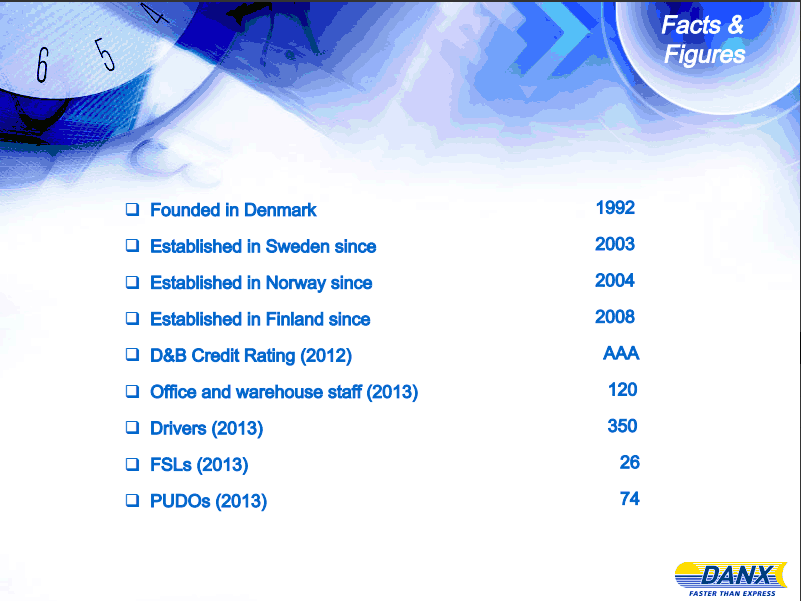
\includegraphics[scale=0.62]{img/DANX_FSL_PUDO}

\bibitem{img002}
	Cost benefit for tailored basic solution\\
	%http://i.imgur.com/rJZnQZi.png
	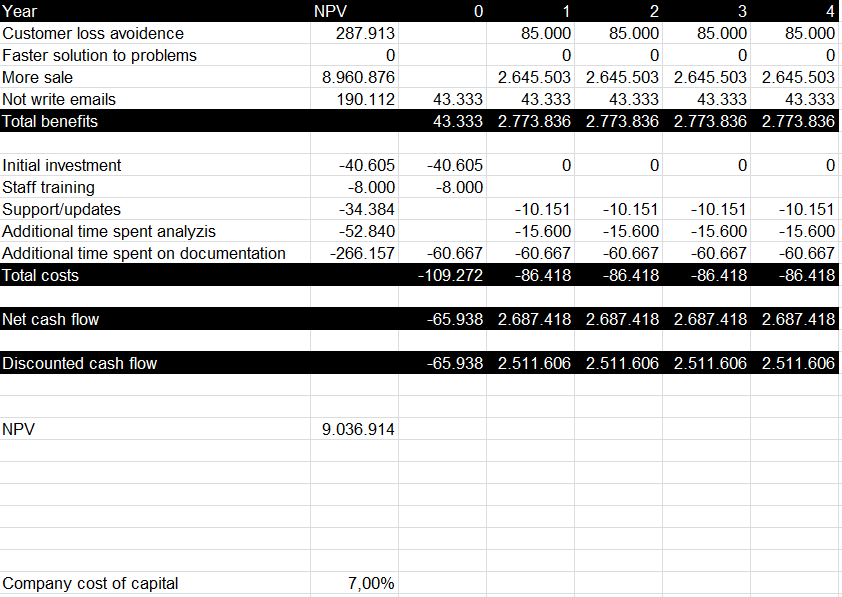
\includegraphics[scale=0.6]{img/CostBenefit_TailoredBasic}

\bibitem{img003}
	Cost benefit for tailored extended system\\
	%http://i.imgur.com/iNIannt.png
	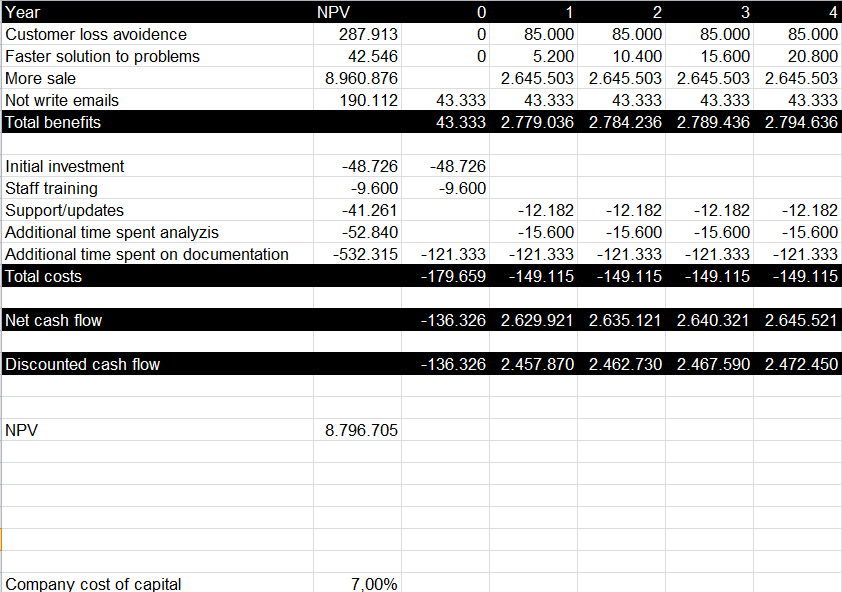
\includegraphics[scale=0.6]{img/CostBenefit_TailoredExtended}

\bibitem{img004}
	Cost benefit for off-the-shelf solution kayako\\
	%http://i.imgur.com/bUaRjPM.png
	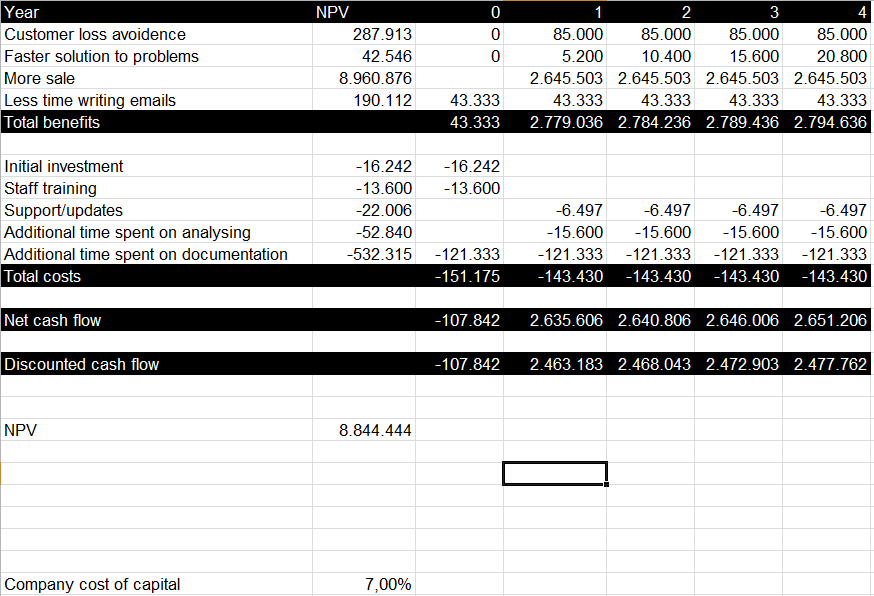
\includegraphics[scale=0.6]{img/CostBenefit_Off-the-shelf}

\end{thebibliography}


\end{document}